\chapter{การออกแบบ และรายละเอียดการพัฒนา}
\label{chapter:experiment}
\section{โครงสร้างและภาพรวมของระบบ}
ระบบจัดการบริหารทรัพยากรบุคคล หรือในชื่อโปรเจค ManyFox พัฒนาขึ้นเพื่อจัดการบริหารภายในองค์กรขนาดเล็ก
โดยระบบที่พัฒนานั้นแบ่งเป็น 6 ส่วน ได้แก่ องค์กรขนาดเล็ก, Slack, เว็บแอปพลิเคชัน (Frontend), ระบบจัดการส่วนหลัง (Backend), Database

\subsection{องค์กรขนาดเล็ก}
องค์กรขนาดเล็กที่มีพนักงาน 2-100คน ที่มีความต้องเก็บข้อมูลพนักงานบน Database มากกว่าในเอกสาร และการจัดการวันลาภายในองค์กรให้มีประสิทธิภาพ
\subsection{Slack}
Slack เป็นแอปพลิเคชันที่ใช้ในการติดต่อสื่อสารกันภายในองค์กร โดยมี Platform ครอบคลุมทั้ง Website, Android, IOS, Windows, Linux และ macOS สมารถสร้าง Channel สำหรับแต่ละหัวข้อได้
และ Slack ยังมีแอปพลิเคชันย่อย ที่ทาง Slack เปิดให้สร้างแอปพลิเคชันย่อยได้ โดยในโปรเจคนี้ จะทำการสร้าง แอปพลิเคชันใน Slack ชื่อ ManyFox

\subsection{เว็บแอปพลิเคชัน (Frontend)}
เว็บแอปพลิเคชัน เป็นส่วนที่เรียกว่า Frontend เป็นส่วนที่ติดต่อกับ User เป็นส่วนที่แสดงข้อมูล การลา ประชุมประจำวัน กิจกรรมต่างๆในองค์กร
หรือดูข้อมูลการลาและจำนวนวันลาที่เหลือของตัวเองได้ และหาก User ที่มีตำแหน่งการบริหาร (ในบริษัท Nextzy technologies คือ C-level Manager และ Senior )
สามารถตอบรับหรือปฎิเสธคำร้องวันลาได้ สามารถเพิ่มลบแก้ไขวันหยุดหรือกิจกรรมในองค์กรได้ สามารถเข้าถึงและแก้ไข ข้อมูลของUserอื่น และสามารถตั้งค่า Workspace ได้ โดยจะเรียกข้อมูลจาก Database จาก API
และนำมาแสดงในหน้า Frontend และเมื่อมี Action ที่ต้องถูกบันทึกลงใน Database ก็จะทำผ่าน API เช่นกัน



\subsection{ระบบจัดการส่วนหลัง (Backend)}
Backend เป็นส่วนจัดการด้านหลัง โดยเชื่อมต่อกับกับ Frontend Slack และ Database โดยแยกเป็น 2 ส่วนดังนี้
\subsubsection{API Web service}
API Web service เป็นส่วนที่เชื่อมต่อกับ Frontend และ Database มีหน้าที่จัดการกับคำร้อง(Request) จาก Frontend
แล้วตรวจสอบประเภทข้อมูล และการอนุญาต ในการอ่าน เพิ่ม ลบ หรือแก้ไขใน Database อาจมีการแปลงรูปแบบข้อมูลก่อนส่งการตอบรับ (Response)
กลับไปหา Frontend

\subsubsection{Slackbot service}
Slackbot service เป็นส่วนที่เชื่อมต่อกับ Slack และ Database  มีหน้าที่จัดการและสร้าง ฟังก์ชั่นที่ถูกประจำในเวลาที่ตั้งไว้ (Cron) ในแต่ละองค์กร สร้างและจัดการ
การตอบสนองอัตโนมัติ (Auto-reply) ในแต่ละองค์กร สร้างและจัดการ หน้าต่าง (Modal) เขียนคำขอร้องลางาน (Off work) หรือ เขียนบันทึกสิ่งต้องทำประจำวัน (Daily meeting)



\section{คุณสมบัติหลักของระบบ}
คุณสมบัติของ ManyFox

\subsection{เข้าสู่ระบบผ่าน Slack}
ผู้ใช้สามารถ เข้าระบบผ่านทางSlackได้ โดยผู้ใช้จำเป็นต้องสร้างหรือมี Workspace ก่อนถึงสามารถใช้งานได้
\subsection{ลงทะเบียน ManyFox}
ผู้ใช้สามรถลงทะเบียน ManyFoxเข้าสู่ Workspace ของ Slack ผ่านทางหน้าเว็บ https://ManyFox.com หรือผ่านทาง Slack โดยกด Add App
ได้โดยผู้ใช้จำเป็นต้องเป็น Administrator ถึงสามารถลงทะเบียนได้

\subsection{เขียนและแก้ไขDaily task}
ผู้ใช้สามารถเขียน ผ่าน Slack โดยพิมพ์คำสั่ง "/task" และมีหน้าต่างแสดงช่องให้พิมพ์สิ่งที่ทำไปแล้ว สิ่งที่กำลังจะทำวันนี้ และ สิ่งที่ต้องทำต่อไปได้และสามารถแก้ไขDaily task ของวันนี้ได้ผ่านการพิมพ์คำสั่ง "/task edit"
\subsection{แสดงผลDaily task}
ผู้ใช้สามารถเรียกดูDaily taskที่ตนเองเขียนได้ เรียงตามวันที่โดยวันล่าสุดขึ้นก่อน หรือสามารถคัดกรองช่วงวันที่ต้องการได้

\subsection{เขียนคำร้องลางานผ่าน Slack}
ผู้ใช้สามรถเขียนคำร้องลางานผ่านทาง Slack โดยพิมพ์คำสั่ง "/offwork" และมีหน้าต่างแสดงให้เลือก ประเภทการลา เหตุผลการลา ระยะเวลาการลา(ทั้งวัน ครึ่งเช้า หรือครึ่งบ่าย) และวันที่ลาได้
และสามารถยกเลิกผ่านทาง Slack โดยการกดปุ่มยกเลิกได้

\subsection{ตอบรับหรือปฎิเสธคำร้องลางาน}
ผู้ใช้ที่มีสิทธิ์ในการตอบรับหรือปฎิเสธคำร้องลางานสามารถกดตอบรับหรือปฎิเสธผ่านหน้าเว็บไซต์ในหน้า Dashboard และหากกดปฎิเสธสามารถกรอกเหตุผลการปฎิเสธได้ เมื่อกดตอบรับหรือปฎิเสธแล้วจะมีแจ้งเตือนถึงผู้เขียนคำร้องได้

\subsection{แสดงผลกราฟการลาภายในบริษัท}
ผู้ใช้ที่มีสิทธิ์ในการตอบรับหรือปฎิเสธคำร้องลางานสามารถเรียกดูกราฟการลาภายในบริษัทภายในปีนี้ได้ สามารถเรียกดูเฉพาะแต่ละเดือนหรือช่วงเดือนได้ และสามารถนำออกมาเป็นไฟล์Excel (.xlsx)ได้

\subsection{จัดการประเภทกิจกรรม}
ผู้ใช้ที่มีสิทธิ์ในการจัดการกิจกรรมภายในองค์กร สามารถเพิ่ม แก้ไขหรือลบประเภทกิจกรรมพร้อมเลือกสีที่จะแสดงในปฎิทิน สามารถเลือกเปิด ปิด ประเภทกิจกรรมที่ต้องการให้แสดงในปฎิทินได้
และสามารถ นำเข้าปฎิทินจาก Pubilc ที่เป็นตัวกลางที่ทาง ManyFox จะจัดการข้อมูลเอง เช่น วันหยุดของประเทศไทย
\subsection{จัดการกิจกรรมภายในบริษัทได้}
ผู้ใช้ที่มีสิทธิในการจัดการกิจกรรมภายในองค์กร สามารถเพิ่ม แก้ไขหรือลบกิจกรรมภายในองค์กร โดยสามารถเขียนชื่อหัวข้อ วันที่ และ ประเภทได้

\subsection{แสดงผลปฎิทินองค์กร}
ผู้ใช้สามารถเรียกดูปฎิทินองค์กร ที่มีข้อมูลวันหยุด-กิจกรรมของบริษัท พนักงานที่ลาในวันนั้น และสามารถเรียกเห็นเฉพาะของตัวเองได้ หรือ เรียกเห็นเฉพาะประเภทการลาได้
\subsection{แสดงผลแจ้งเตือนเหตุการณ์}
ผู้ใช้สามารถเรียกดูการแจ้งเตือนเหตุการณ์ภายในองค์กร เช่น มีบุคคลอนุญาต/ปฎิเสธการลาของตนและเหตุผล และมีการเพิ่มหรือแก้ไขปฎิทินองค์กร เป็นต้น

\subsection{แสดงผลข้อมูลพนักงานและข้อมูลส่วนตัวของตนเอง}
ผู้ใช้สามารถเรียกดูข้อมูลพนักงานของตนเอง (ชื่อ ตำแหน่ง ระดับชั้น และรูปแบบการจ้างงาน) ข้อมูลส่วนตัวของพนักงาน ข้อมูลของจำนวนการลาของผู้ใช้ในปีนี้ และวันลาพักร้อนที่เหลืออยู่
\subsection{แสดงผลข้อมูลพนักงานและข้อมูลส่วนตัวภายในบริษัท}
ผู้ใช้ที่มีสิทธิในการจัดการข้อมูลพนักงาน สามารถเรียกดูข้อมูลพนักงานภายในบริษัท (ชื่อ ตำแหน่ง ระดับชั้น และรูปแบบการจ้างงาน) ข้อมูลส่วนตัวของพนักงาน
ข้อมูลของจำนวนการลาของผู้ใช้ในปีนี้ และวันลาพักร้อนที่เหลืออยู่ และสามารถเรียกดูเฉพาะตามตำแหน่งตามที่ต้องการได้
\subsection{แสดงผลกราฟข้อมูลการลาของพนักงาน}
ผู้ใช้ที่มีสิทธิในการจัดการข้อมูลพนักงาน สามารถเรียกดูกราฟแท่งแสดงข้อมูลการลาของพนักงาน โดยแบ่งตามสีได้ สามารถเลือกดูปีย้อนหลังได้ และสามารถนำออกมาเป็นไฟล์Excel (.xlsx)ได้
\subsection{จัดการข้อมูลพนักงาน}
ผู้ใช้ที่มีสิทธิในการจัดการข้อมูลพนักงาน สามารถแก้ไขข้อมูล ตำแหน่ง ระดับชั้น รูปแบบการจ้างงาน และวันที่เริ่มทำงานของพนักงานภายในบริษัทได้
\subsection{จัดการข้อมูลส่วนตัวได้}
ผู้ใช้สามารถแก้ไขข้อมูลส่วนตัว (เพศ ปีเกิด ที่อยู่ และเบอร์โทร)ของตนเองได้
\subsection{ค้นหาข้อมูลพนักงาน}
ผู้ใช้ที่มีสิทธิในการจัดการข้อมูลพนักงาน สามารถค้นหาข้อมูลพนักงานโดยค้นหาจากชื่อพนักงานได้



\subsection{ตั้งค่าคำตอบสนองแก่คำที่กำหนดไว้อัตโนมัติ}
ผู้ใช้ที่มีสิทธิ์ในการจัดการองค์กร สามารถตั้งค่าคำที่ต้องการให้Bot ตรวจเจอแล้วคำที่ตั้งค่าไว้กลับไป ผ่านทางเว็บไซต์ในหน้า Workspace Setting
\subsection{ตั้งค่าแจ้งเตือนผู้ไม่เขียนDaily task}
ผู้ใช้ที่มีสิทธิ์ในการจัดการองค์กร สามารถตั้งค่าให้แจ้งเตือนแท๊กผู้ที่ไม่เขียนDaily task ในเวลาที่กำหนดผ่านทางเว็บไซต์ Workspace Setting สามารถใส่หรือแก้ไขข้อความต่อท้ายได้ และสามารถเลือก Channel ที่จะแจ้งเตือนได้
\subsection{ตั้งค่าแจ้งเตือนพนักงานที่ลาวันนี้ได้}
ผู้ใช้ที่มีสิทธิ์ในการจัดการองค์กร สามารถตั้งค่าให้แจ้งเตือนพนักงานที่ลาวันนี้ในเวลาที่กำหนดผ่านทางเว็บไซต์ Workspace Setting และสามารถเลือก Channel ที่จะแจ้งเตือนได้
\subsection{ตั้งค่าการลาของพนักงาน}
ผู้ใช้ที่มีสิทธิ์ในการจัดการองค์กร สามารถตั้งค่าประเภทการลาที่ของพนักงานที่สามารถลาได้ตามรูปแบบการจ้างงาน สามารถตั้งค่าประเภทการลาที่ต้องแจ้งก่อนเท่าใด หรือสามารถตั้งค่าจำนวนการของประเภทการลาเท่าใด
\subsection{ตั้งค่ารูปแบบการจ้างานของพนักงาน}
ผู้ใช้ที่มีสิทธิ์ในการจัดการองค์กร สามารถตั้งค่าเพิ่ม แก้ไข หรือลบรูปแบบการจ้างงาน เช่น พนักงานเงินเดือน, นักศึกษาฝึกงาน และ พนักงานอิสระ เป็นต้น
\subsection{ตั้งค่าระดับชั้นของพนักงาน}
ผู้ใช้ที่มีสิทธิ์ในการจัดการองค์กร สามารถตั้งค่าเพิ่ม แก้ไข หรือลบระดับชั้นของพนักงาน และกำหนดสิทธิ์การเข้าถึงของแต่ละระดับชั้นได้
\subsection{ตั้งค่าตำแหน่งของพนักงาน}
ผู้ใช้ที่มีสิทธิ์ในการจัดการองค์กร สามารถตั้งค่าเพิ่ม แก้ไข หรือลบตำแหน่งของพนักงาน เช่น Web Developer, UX/UI Designer, System Analyst และ Business Analyst เป็นต้น
\section{ขั้นตอนการพัฒนา}

การพัฒนาโปรเจคจะแบ่งตาม Sprint โดย 1 sprint จะมีระยะเวลา 2-4 สัปดาห์ ภายในทีมประกอบไปด้วย Project manager, System Analyst, UX/UI Designer, Tester และ Web Developer
โดยการจัดการวางแผน Sprint การเก็บ Requirement และการแบ่งงานเป็นหน้าที่ของ Project manager และ System Analyst โดยเริ่มต้นจาก UX/UI Designer ออกแบบ UI interface ของแต่ละ Page หรือ Feature
เพื่อส่งต่อให้ Web Developer นำไปพัฒนาใน Sprint ต่อไป และเมื่อพัฒนาเสร็จ จะส่งต่อให้ Tester ทดสอบเพื่อจุดบกพร่องใน Sprint ต่อไป
\newpage
\begin{table}[!htbp]
	\centering
	\begin{tabular}{|c|c|c|c|}
		\hline
		\textbf{Sprint}  & Sprint2                   & Sprint 3                  & Sprint 4                  \\ \hline
		\textbf{Feature} & \begin{tabular}[c]{@{}c@{}}Profile\\ Calendar\\ Dashboard\\ Individual Report\\ /task command\\ /offwork command\end{tabular} & \begin{tabular}[c]{@{}c@{}}All profile\\ Edit profile\\ /whooffworks command\end{tabular} & \begin{tabular}[c]{@{}c@{}}Mayfox Install\\ Authentication\\ Notifications\end{tabular} \\ \hline
		\textbf{Sprint}  & Sprint 5                  & Sprint 6                  & Sprint 7                  \\ \hline
		\textbf{Feature} & \begin{tabular}[c]{@{}c@{}}Landing page\\ Feedback\\ Search users\end{tabular} & Leave Setting             & \begin{tabular}[c]{@{}c@{}}All profile\\ Edit profile\\ /whooffworks command\end{tabular} \\ \hline
		\textbf{Sprint}  & Sprint 8                  &                           &                           \\ \hline
		\textbf{Feature} & \begin{tabular}[c]{@{}c@{}}Mayfox Install\\ Authentication\\ Notifications\end{tabular} &                           &                           \\ \hline
	\end{tabular}
	\caption{Sprint plan}
\end{table}


\vskip1em เนื่องจากโปรเจคนี้เริ่มพัฒนาตั้งแต่ช่วงที่นักศึกษาฝึกงานและมีพนักงานร่วมพัฒนา โดยงานที่นักศึกษารับผิดชอบในที่ส่วน Frontend ของ Client ในช่วงฝึกงาน
และรับผิดชอบทั้ง Frontend และ Backend ในช่วงสหกิจ โดยมีการแบ่งหน้าที่รับผิดชอบและงานที่ได้รับมอบหมายดังที่ ปรากฎในตาราง
\begin{table}[!htbp]
	\centering
	\begin{tabular}{cccl}
		\hline
		\multicolumn{1}{|c|}{\textbf{ManyFox System}} & \multicolumn{1}{c|}{\textbf{ผู้รับผิดชอบ Frontend}} & \multicolumn{1}{c|}{\textbf{ผู้รับผิดชอบ Backend}} \\ \hline
		\multicolumn{1}{|c|}{ManyFox Install}         & \multicolumn{1}{c|}{นักศึกษา}                     & \multicolumn{1}{c|}{พนักงาน}                    \\ \hline
		\multicolumn{1}{|c|}{Authentication}          & \multicolumn{1}{c|}{นักศึกษา}                     & \multicolumn{1}{c|}{พนักงาน }                   \\ \hline
		\multicolumn{1}{|c|}{Profile}                 & \multicolumn{1}{c|}{นักศึกษา}                     & \multicolumn{1}{c|}{นักศึกษา \& พนักงาน}          \\ \hline
		\multicolumn{1}{|c|}{Edit profile}            & \multicolumn{1}{c|}{นักศึกษา \& พนักงาน}           & \multicolumn{1}{c|}{นักศึกษา \& พนักงาน}          \\ \hline
		\multicolumn{1}{|c|}{All profile}             & \multicolumn{1}{c|}{นักศึกษา}                     & \multicolumn{1}{c|}{พนักงาน}                    \\ \hline
		\multicolumn{1}{|c|}{Calendar}                & \multicolumn{1}{c|}{นักศึกษา}                     & \multicolumn{1}{c|}{พนักงาน}                    \\ \hline
		\multicolumn{1}{|c|}{Individual Report}       & \multicolumn{1}{c|}{นักศึกษา \& พนักงาน}           & \multicolumn{1}{c|}{พนักงาน}                    \\ \hline
		\multicolumn{1}{|c|}{Daily task}              & \multicolumn{1}{c|}{นักศึกษา}                     & \multicolumn{1}{c|}{นักศึกษา}                    \\ \hline
		\multicolumn{1}{|c|}{Search users}            & \multicolumn{1}{c|}{นักศึกษา \& พนักงาน}           & \multicolumn{1}{c|}{พนักงาน}                    \\ \hline
		\multicolumn{1}{|c|}{Dashboard}               & \multicolumn{1}{c|}{นักศึกษา}                     & \multicolumn{1}{c|}{พนักงาน}                    \\ \hline
		\multicolumn{1}{|c|}{Leave Setting}           & \multicolumn{1}{c|}{พนักงาน}                     & \multicolumn{1}{c|}{พนักงาน}                    \\ \hline
	\end{tabular}
\end{table}

\begin{table}[!htbp]
	\centering
	\begin{tabular}{cccl}
		\hline
		\multicolumn{1}{|c|}{\textbf{ManyFox System}}      & \multicolumn{1}{c|}{\textbf{ผู้รับผิดชอบ Frontend}} & \multicolumn{1}{c|}{\textbf{ผู้รับผิดชอบ Backend}} \\ \hline
		\multicolumn{1}{|c|}{Bot Setting}                  & \multicolumn{1}{c|}{นักศึกษา}                     & \multicolumn{1}{c|}{นักศึกษา}                    \\ \hline
		\multicolumn{1}{|c|}{User Setting}                 & \multicolumn{1}{c|}{พนักงาน}                     & \multicolumn{1}{c|}{พนักงาน}                    \\ \hline
		\multicolumn{1}{|c|}{Feedback}                     & \multicolumn{1}{c|}{นักศึกษา}                     & \multicolumn{1}{c|}{พนักงาน}                    \\ \hline
		\multicolumn{1}{|c|}{Master Calendar Setting}      & \multicolumn{1}{c|}{พนักงาน}                     & \multicolumn{1}{c|}{พนักงาน}                    \\ \hline
		\multicolumn{1}{|c|}{Notifications}                & \multicolumn{1}{c|}{นักศึกษา}                     & \multicolumn{1}{c|}{พนักงาน}                    \\ \hline
		\multicolumn{1}{|c|}{/offwork command}             & \multicolumn{1}{c|}{-}                          & \multicolumn{1}{c|}{พนักงาน}                    \\ \hline
		\multicolumn{1}{|c|}{/whooffworks command}         & \multicolumn{1}{c|}{-}                          & \multicolumn{1}{c|}{พนักงาน}                    \\ \hline
		\multicolumn{1}{|c|}{/task command}                & \multicolumn{1}{c|}{-}                          & \multicolumn{1}{c|}{พนักงาน}                    \\ \hline
		\multicolumn{1}{|c|}{/meeting command}             & \multicolumn{1}{c|}{-}                          & \multicolumn{1}{c|}{พนักงาน}                    \\ \hline
		\multicolumn{1}{|c|}{Auto increase remain offwork} & \multicolumn{1}{c|}{-}                          & \multicolumn{1}{c|}{พนักงาน}                    \\ \hline
		\multicolumn{1}{|c|}{Landing page}                 & \multicolumn{1}{c|}{นักศึกษา}                     & \multicolumn{1}{c|}{-}                         \\ \hline
	\end{tabular}
	\caption{ตารางการมอบหมายงาน}
\end{table}

\subsection{ManyFox Install}
ในการลงทะเบียนติดตั้งใช้งาน Manyfox จำเป็นต้องมี Slack workspace และมิสิทธิ์เป็น Owner หรือ Administrator ใน Slack workspace นั้นถึงสามารถติดตั้งได้
โดยแบ่งออกเป็น 5 ขั้นตอนดังนี้
\subsubsection{introduction}
หน้าแรกสำหรับเข้าสู่การลงทะเบียน เมือกด ADD TO SLACK หากล๊อกอิน Slack ในบราวเซอร์
จะเข้าสู่หน้า Request permission แต่หากไม่ได้ล๊อกอินจะเข้าสู่หน้า Slack login
\begin{figure}[!htbp]
	\centering
	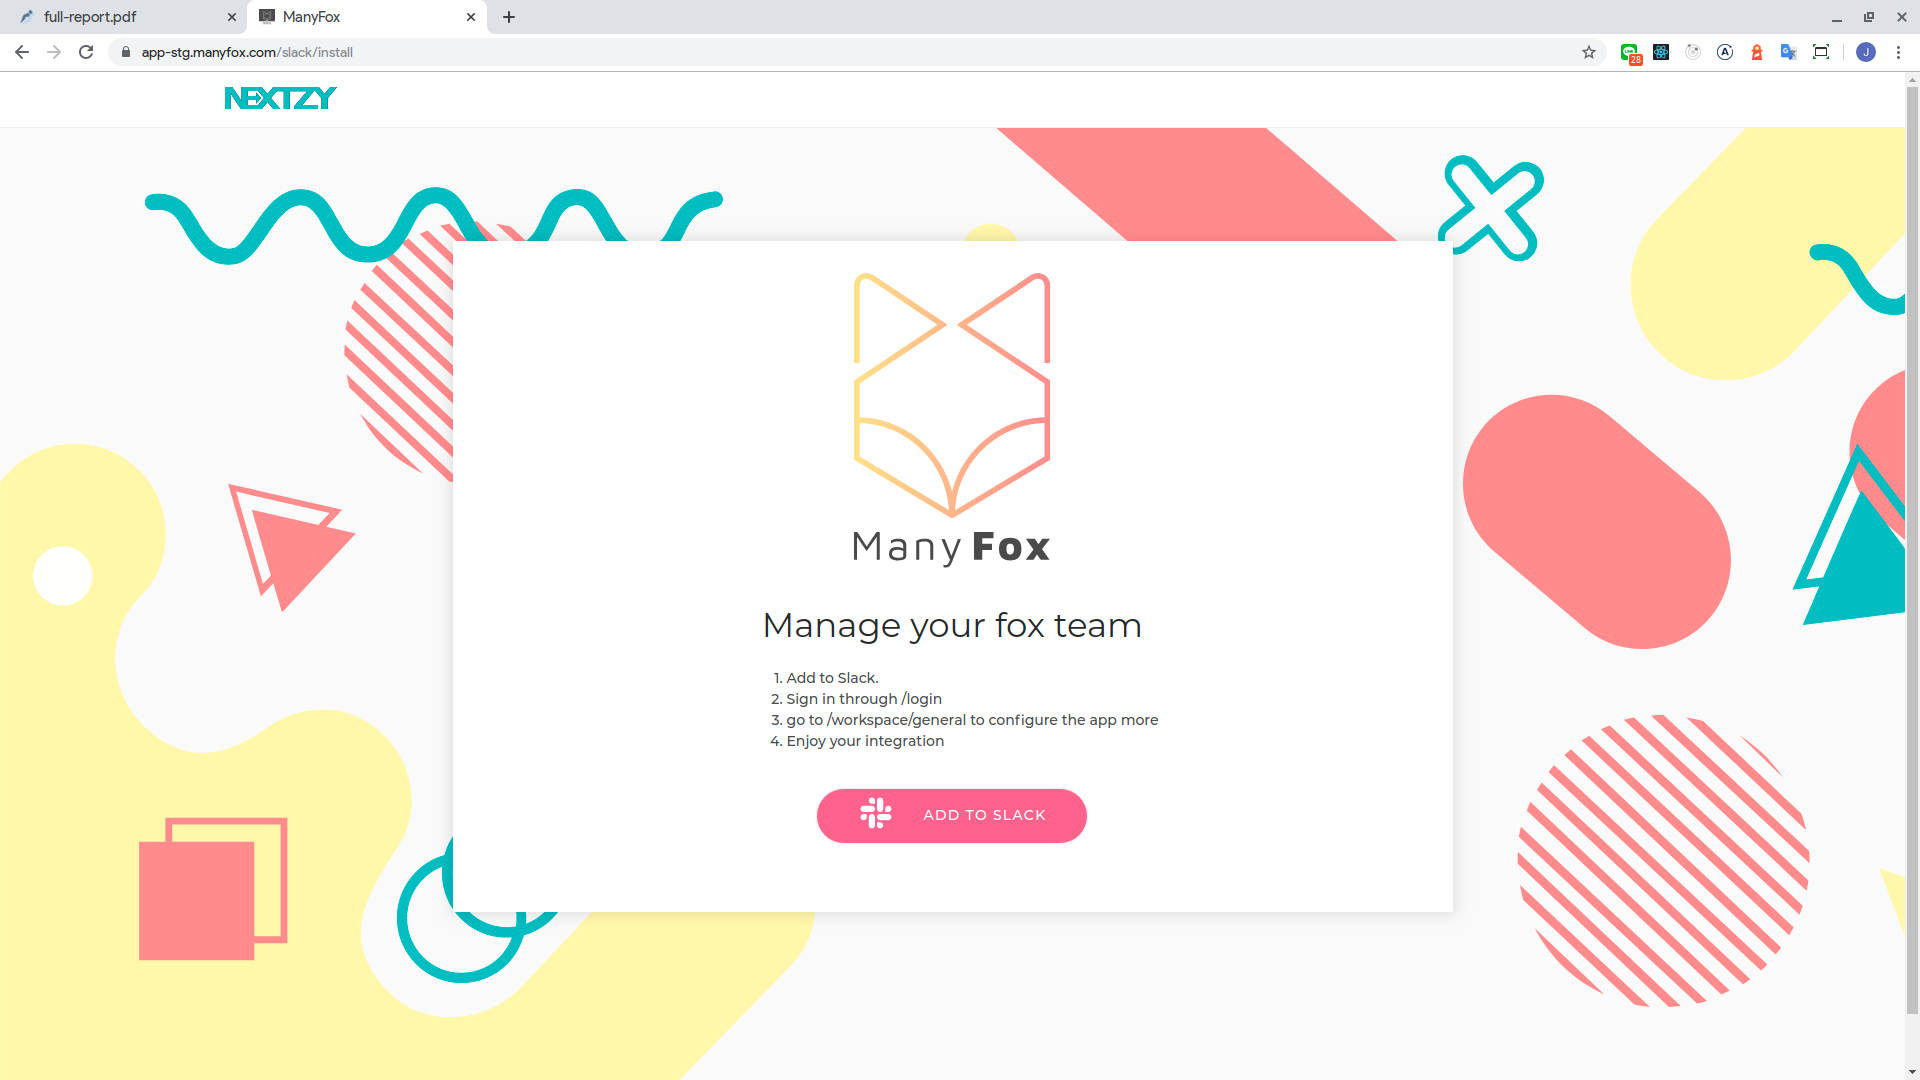
\includegraphics[width=0.8\linewidth]{install-1}
	\caption{introduction}
	\label{Fig:introduction}
\end{figure}
\subsubsection{Slack Login}
Slack login หน้าแรกจะให้กรอก workspace url ของ บริษัท ก่อนเมื่อกด Continue
ระบบจะนำไปตรวจสอบหาว่ามี workspace url นี้จริงหรือไม่ หากมีจะเข้าสู่หน้า Sign in to { \textbf{your Workspace} }
จะมีให้กรอก email และ password ของพนักงานโดย email ของพนักงานจำเป็นต้องอยู่ใน
workspace ของบริษัทเพื่อเข้าสู่ระบบของ Slack และไปในหน้า Request permission ต่อไป
\begin{figure}[!htbp]
	\centering
	\subfigure[Sign in workspace]{
		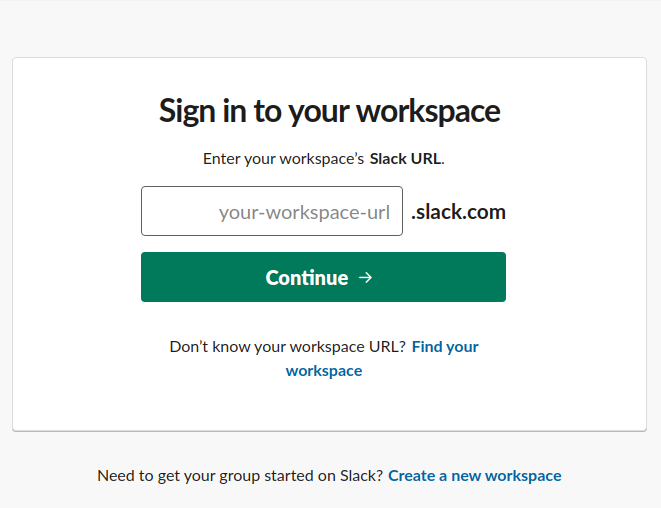
\includegraphics[width=0.45\linewidth]{install-2}
		\label{Fig:slack-login-1}
	}
	\subfigure[Sign in email]{
		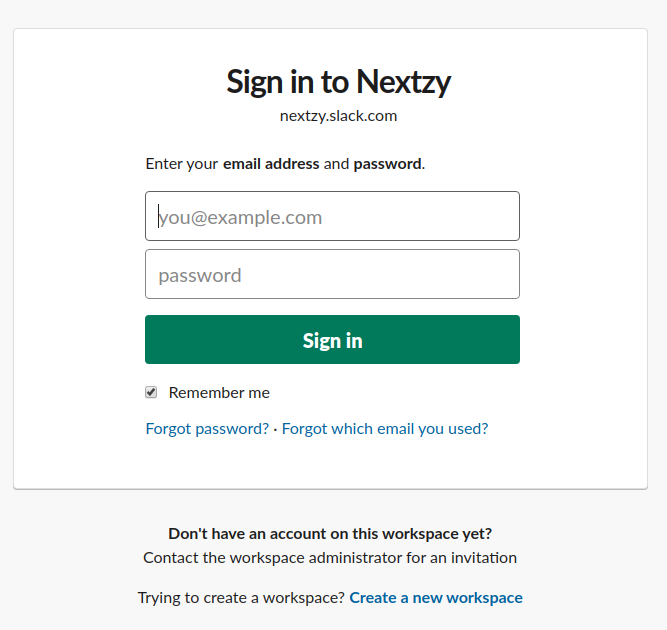
\includegraphics[width=0.45\linewidth]{install-3}
		\label{Fig:slack-login-2}
	}
	\caption{slack login}

\end{figure}
\subsubsection{Request permission}
แอปพลิเคชัน Manyfox จะแสดงคำร้องของการเข้าถึงข้อมูลภายใน Slack
\begin{figure}[!htbp]
	\centering
	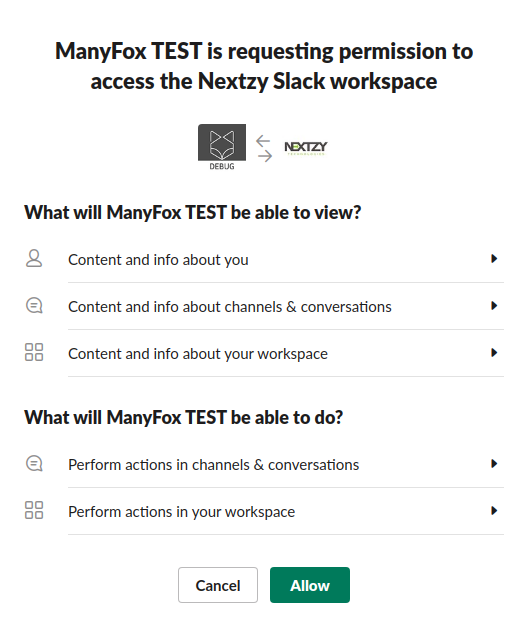
\includegraphics[width=0.4\linewidth]{install-4}
	\caption{Request permission}
	\label{Fig:permission}
\end{figure}
\subsubsection{Create initial database}
จะเป็นหน้า Redirect เพื่อยิง API ให้ Backend ดึงข้อมูลจาก Slack มาสร้าง Workspace ภายใน Database
\subsubsection{Install Success}
หากการสร้าง Workspaceเสร็จสิ้น จะขึ้นข้อความ Successfully และเมื่อกดปุ่ม Sign in With Slack จะทำการ Sign in ไปยัง Workspace อัตโนมัติ
\begin{figure}[!h]
	\centering
	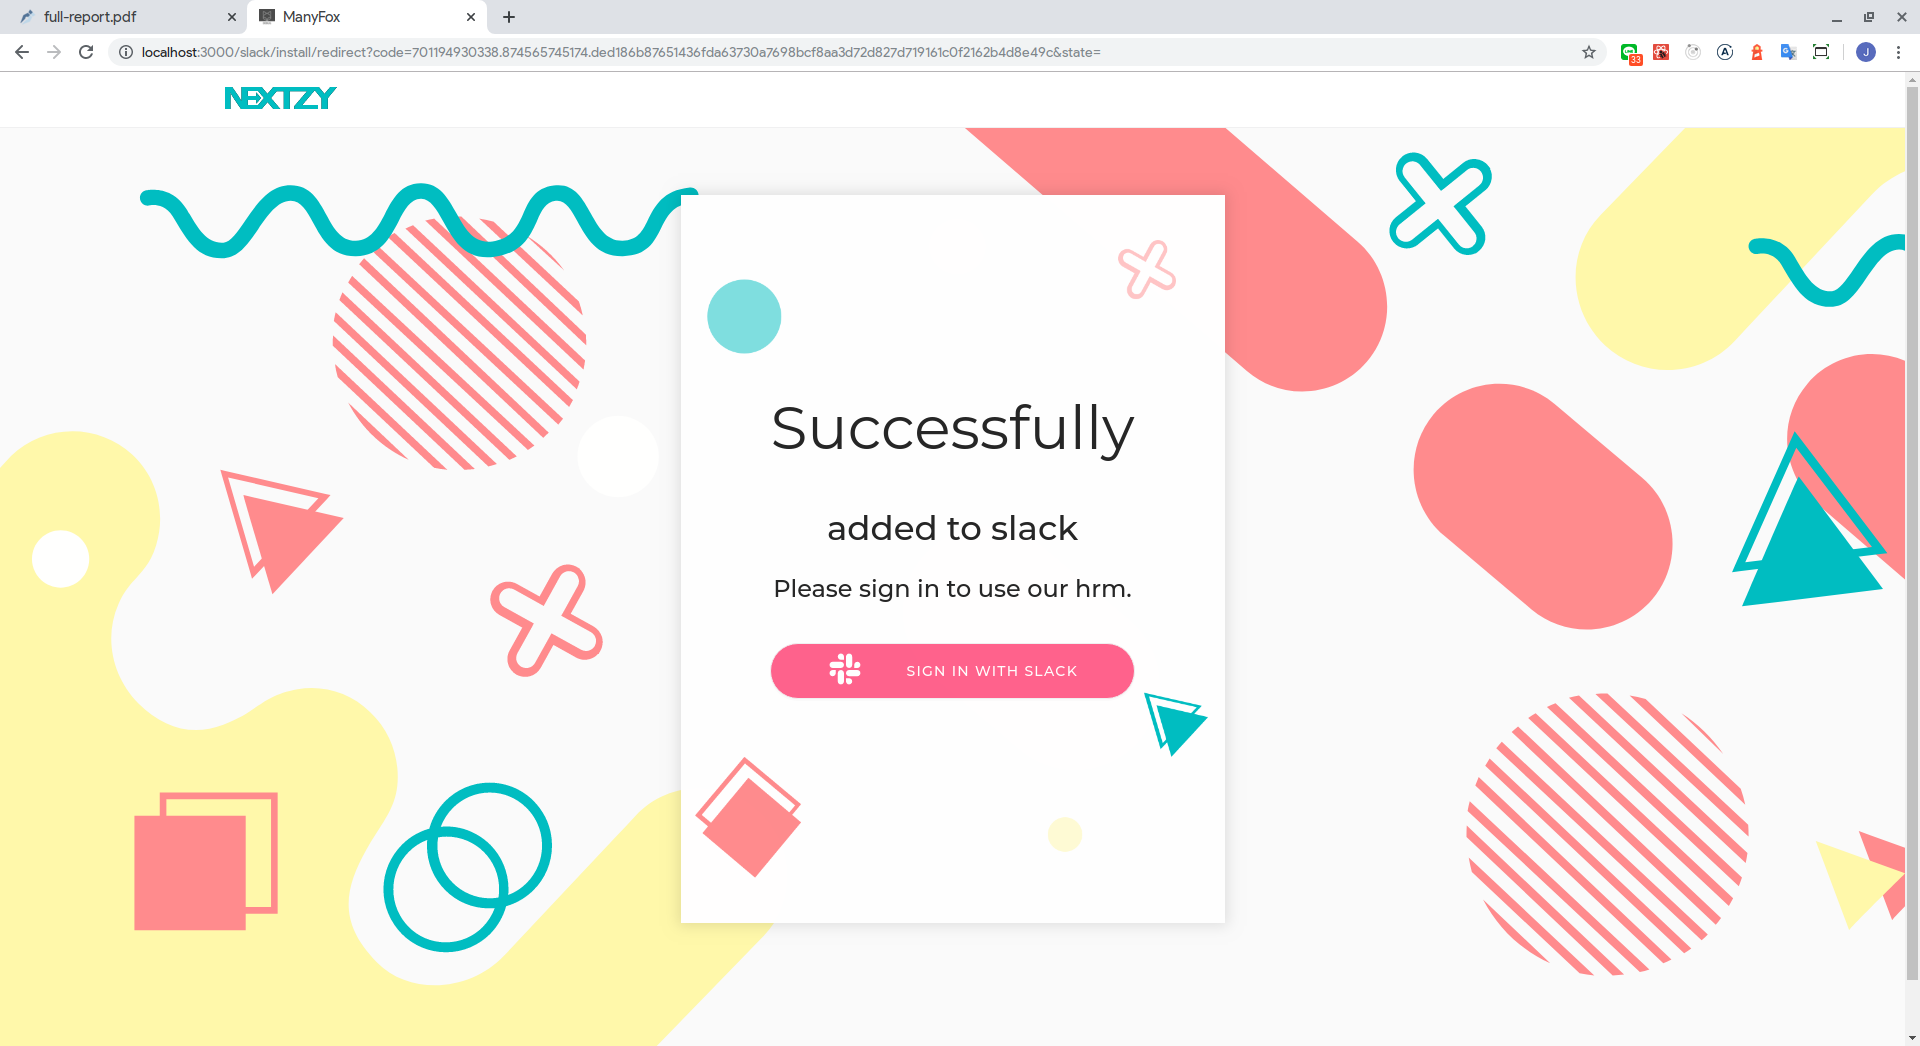
\includegraphics[width=0.7\linewidth]{install-5}
	\caption{Install Success}
	\label{Fig:success}
\end{figure}

\subsection{Authentication}
เมื่อสร้าง Workspace ใน Manyfox เสร็จสิ้น สมาชิกทุกใน slack workspace จะสามารถเข้าสู่ระบบภายใต้ workspace ตัวเองได้

\subsection{Profile}
ในส่วน component Profile จะแสดงข้อมูลของ User โดยจะแสดง รูปโปรไฟล์ ชื่อ ตำแหน่ง ระดับชั้น รูปแบบการจ้างงาน สถานะ
จำนวนวันลาของการลาแต่ละประเภทโดยอิงตาม  และแทบสถานะการลาพักร้อน
\vskip1em
โดยด้านขวาบนของ component Profile ยังแบ่งเป็น 2ส่วน ส่วนแรกเป็น สัญลักษณ์ จุด3จุด เมื่อกดจะมี Menu Edit โผล่ออกมาให้เลือก เมื่อกดที่ Edit หน้าข้อมูล Profile จะเปลี่ยนเป็น Edit profile
ส่วนที่2อยู่ด้านล่างของส่วนแรก มีรูปแบบ 2 รูปแบบดังนี้
\vskip1emรูปแบบ \textbf{remain} จะแสดง จำนวนวันลาพักร้อนที่เหลืออยู่

\begin{figure}[!h]
	\centering
	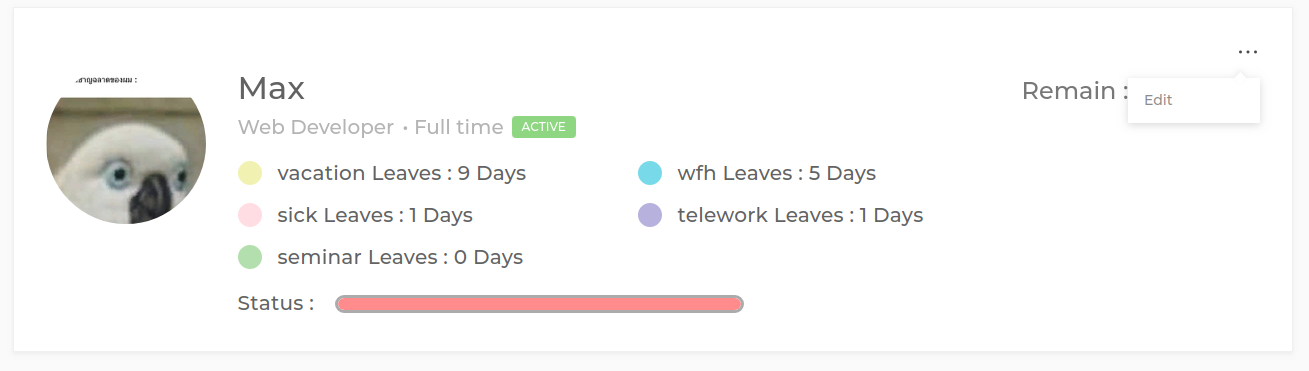
\includegraphics[width=1\linewidth]{profile-remain}
	\caption{Profile รูปแบบ remain}
	\label{Fig:profile-remain}
\end{figure}
\vskip1emรูปแบบ \textbf{more-detail} จะแสดงปุ่ม \textbf{More Detail}" ที่จะลิ๊งไปยัง
/individualreport/\{ \textbf{UserId} \} หน้า Individual report ของ user คนนั้น
\begin{figure}[!h]
	\centering
	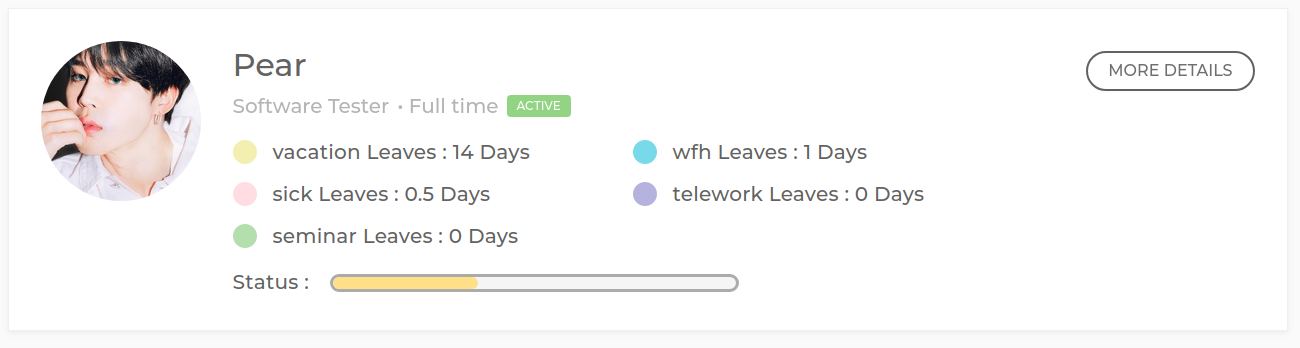
\includegraphics[width=1\linewidth]{profile-more}
	\caption{Profile รูปแบบ more-detail}
	\label{Fig:profile-more}
\end{figure}
\\โดยใช้ GraphQL ในการเรียก API จากฝั่ง Backend และชนิดข้อมูลที่ได้ดังนี้\
\subsection{Edit profile}
หลังจากที่เลือก Edit ในหน้า Profile จะเข้าสู่ component Edit profile จะขึ้นรูป โปรไฟล์ User และช่องกรอกข้อความของ ตำแหน่ง ระดับชั้น
รูปแบบการจ้างงาน เพศ วันเกิด ที่อยู่ เบอร์โทร และวันที่เริ่มทำงานของพนักงาน โดยมีข้อมูลเดิมในช่องอยู่แล้ว เมื่อกด Submit จะบันทึกข้อมูลทับของเก่า และ component กลับไปเป็น Profile
\begin{figure}[!htbp]
	\centering
	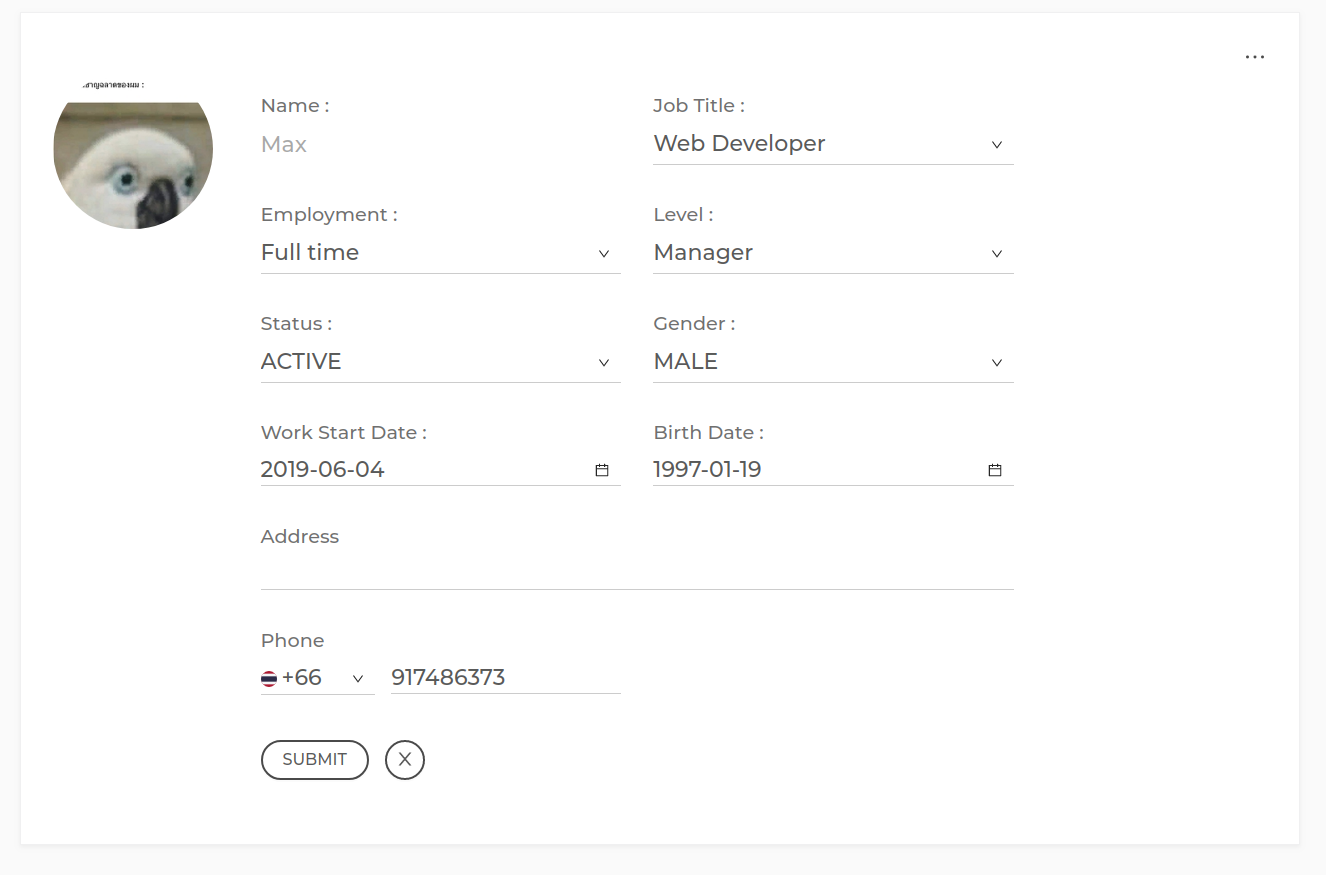
\includegraphics[width=1\linewidth]{edit-profile}
	\caption{Edit Profile}
	\label{Fig:edit-profile}
\end{figure}
\\โดยใช้ GraphQL ในการเรียก API จากฝั่ง Backend ได้ดังนี้


\subsection{All profile}
ในหน้า All profile จะสามารถเข้าถึงเฉพาะระดับชั้นที่มี permission "see\_report" เท่านั้น
โดยจะแสดง component Profile ในรูปแบบ "more-detail" ของพนักงานทุกคนใน Workspace
โดยสามารถ filter ตามตำแหน่ง และสถานะได้
\begin{figure}[!htbp]
	\centering
	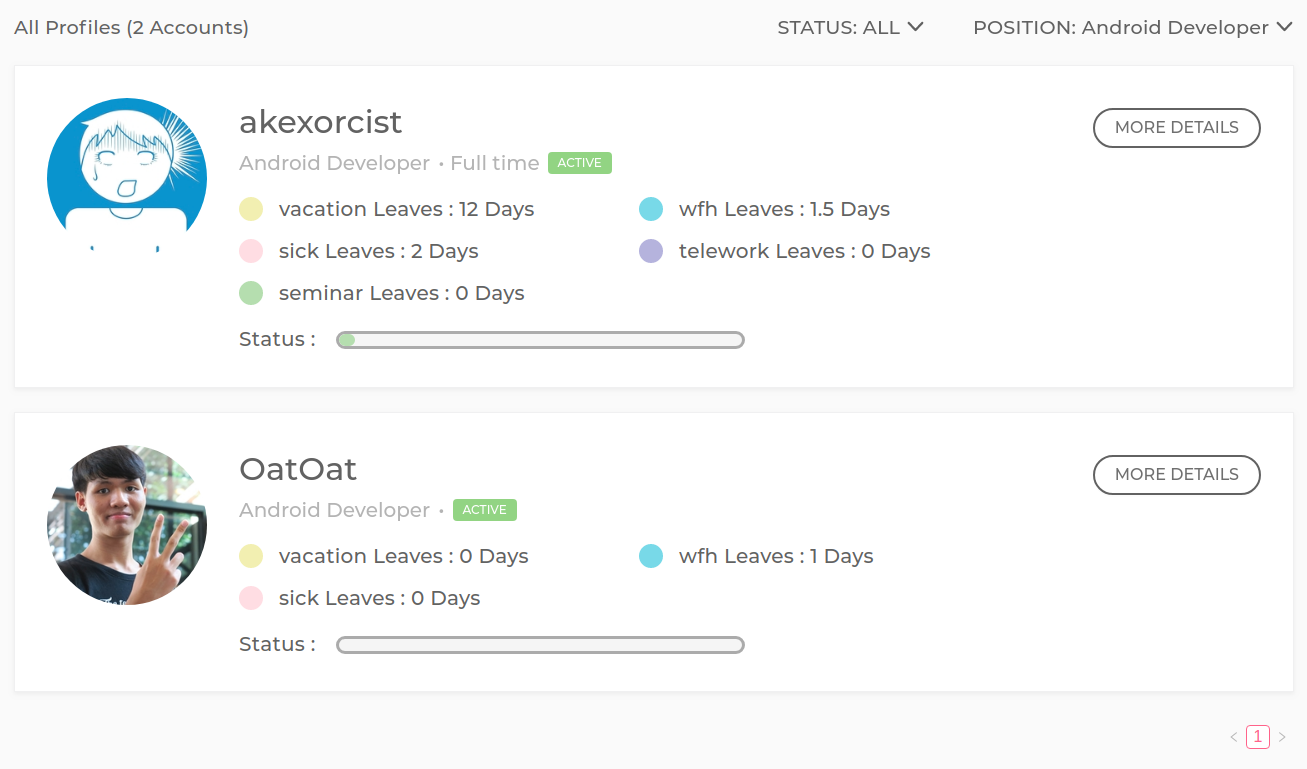
\includegraphics[width=1\linewidth]{all-profile}
	\caption{All profile}
	\label{Fig:all-profile}
\end{figure}
\subsection{Calendar}
Calendar เป็น component ที่ใช้งานทั้งในหน้า Calendar page และ Dashboard page
\vskip1emในหน้า Calendar page จะเป็น Calendar ที่แสดง
event เป็นสีพื้นหลังวันที่ และแสดง ประเภทการลาที่มีในวันนั้นเป็นจุดสี ด้านใต้วันที่
และเมื่อกดที่วันที่จะแสดงข้อมูลวันที่ Event ในวันนั้น และ บุคคลคนที่ลาในวันนั้น พร้อมประเภทการลา และเหตุผล ปรากฎด้านขวามือของ Calendar

\begin{figure}[!htbp]
	\centering
	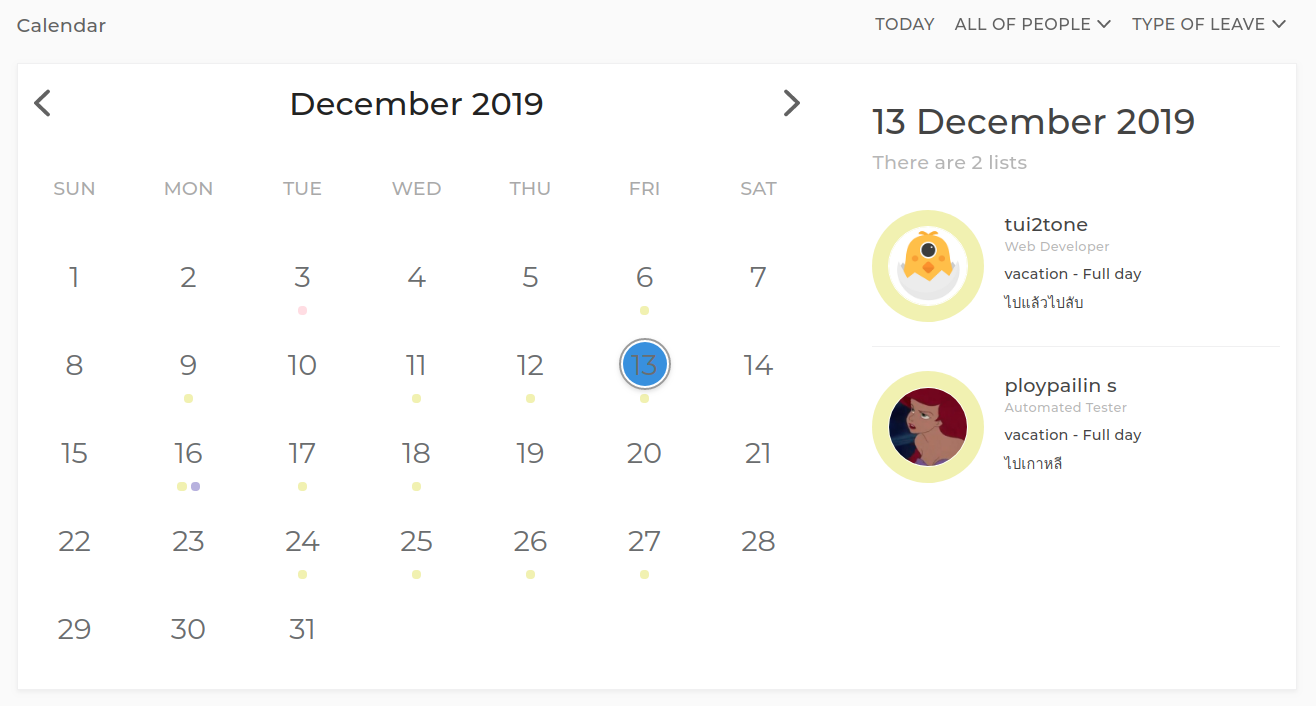
\includegraphics[width=1\linewidth]{calendar-calendar}
	\caption{Calendar ในหน้า Calendar}
	\label{Fig:calendar-calendar}
\end{figure}
\vskip1emในหน้า Dashboard page จะแสดงเฉพาะ event เป็นพื้นหลังวันที่ และเมื่อกดที่วันที่ จะแสดงกล่อง Calendar Modal ขึ้น
\begin{figure}[!htbp]
	\centering
	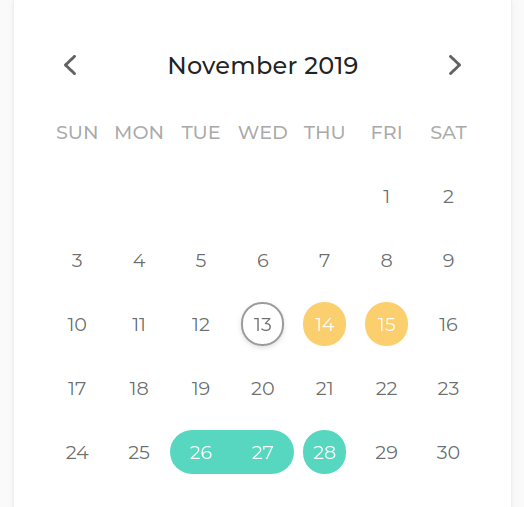
\includegraphics[width=0.5\linewidth]{calendar-dashboard}
	\caption{All ในหน้า Dashboard}
	\label{Fig:calendar-dashboard}
\end{figure}
\subsection{Individual Report}
Individual Report page สามารถเข้าถึงเฉพาะระดับชั้นที่มี permission "see\_report" เท่านั้น
โดยจะแสดง component Profile รูปแบบ "remain" และ Individual Report ของพนักงาน โดยดูจาก UserId
ของพนักงานจาก path "/individualreport/\{ \textbf{UserId} \}"
\vskip1em
ส่วน component Individual Report จะแสดง กราฟแท่งจำนวนวันลาในแต่ละประเภทที่ใช้ใน1ปี โดยแบ่งตามเดือน
และแสดง จำนวนลาที่ใช้ใน1ปีทุกประเภท และแต่ละประเภท และสามารถดูย้อนหลังถอยหลัง 2 ปีได้ และปุ่ม Export

\begin{figure}[!htbp]
	\centering
	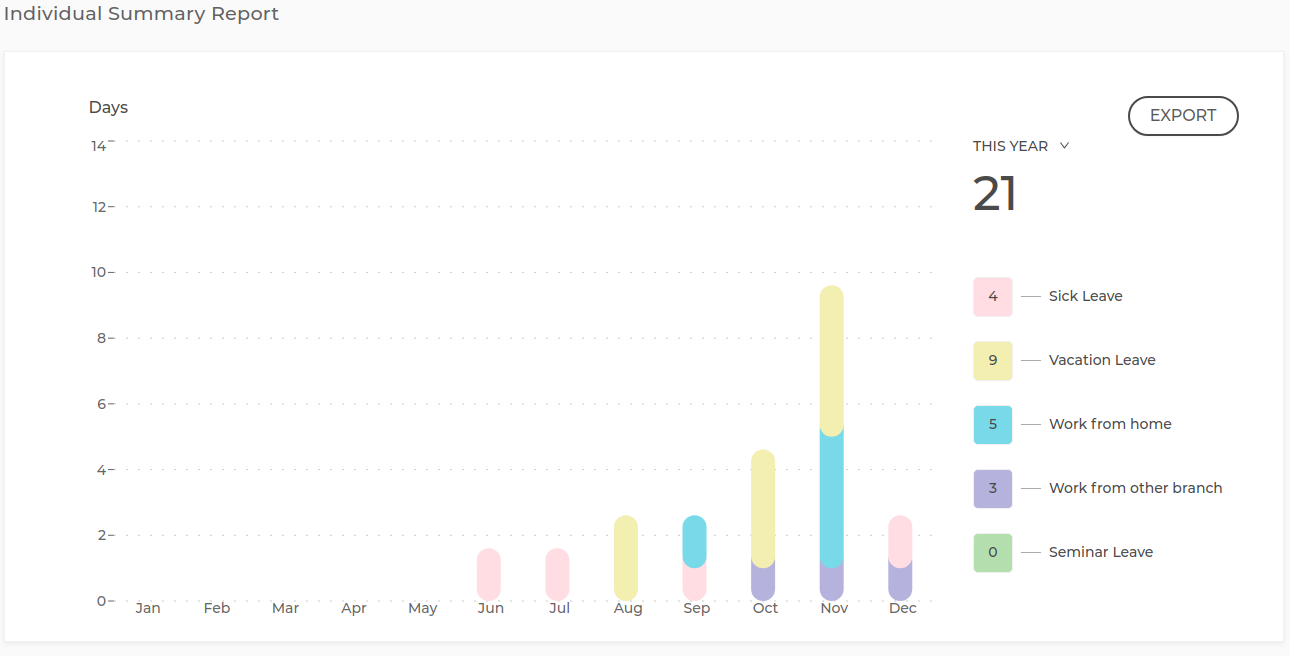
\includegraphics[width=1\linewidth]{individual-report}
	\caption{All ในหน้า Dashboard}
	\label{Fig:individual-report}
\end{figure}
\vskip1em
ปุ่ม Export เมื่อกดจะดาวโหลดไฟล์ตาราง excel (\.xlsx) ข้อมูลการลาของปีที่เลือกอยู่ โดยจะแสดง วันที่ลา ระยะเวลาการลา ประเภทการลา เหตุผลการลา และการได้อนุมัติ/ปฎิเสธ
\subsection{Daily task}
Daily task เป็น component ที่ใช้ในหน้า Daily task จะแสดงข้อมูลการเขียน daily task ในแต่ละวัน โดยแสดงเฉพาะวันจันทร์-ศุกร์และเรียงจากวันล่าสุดลงไป
\begin{figure}[!htbp]
	\centering
	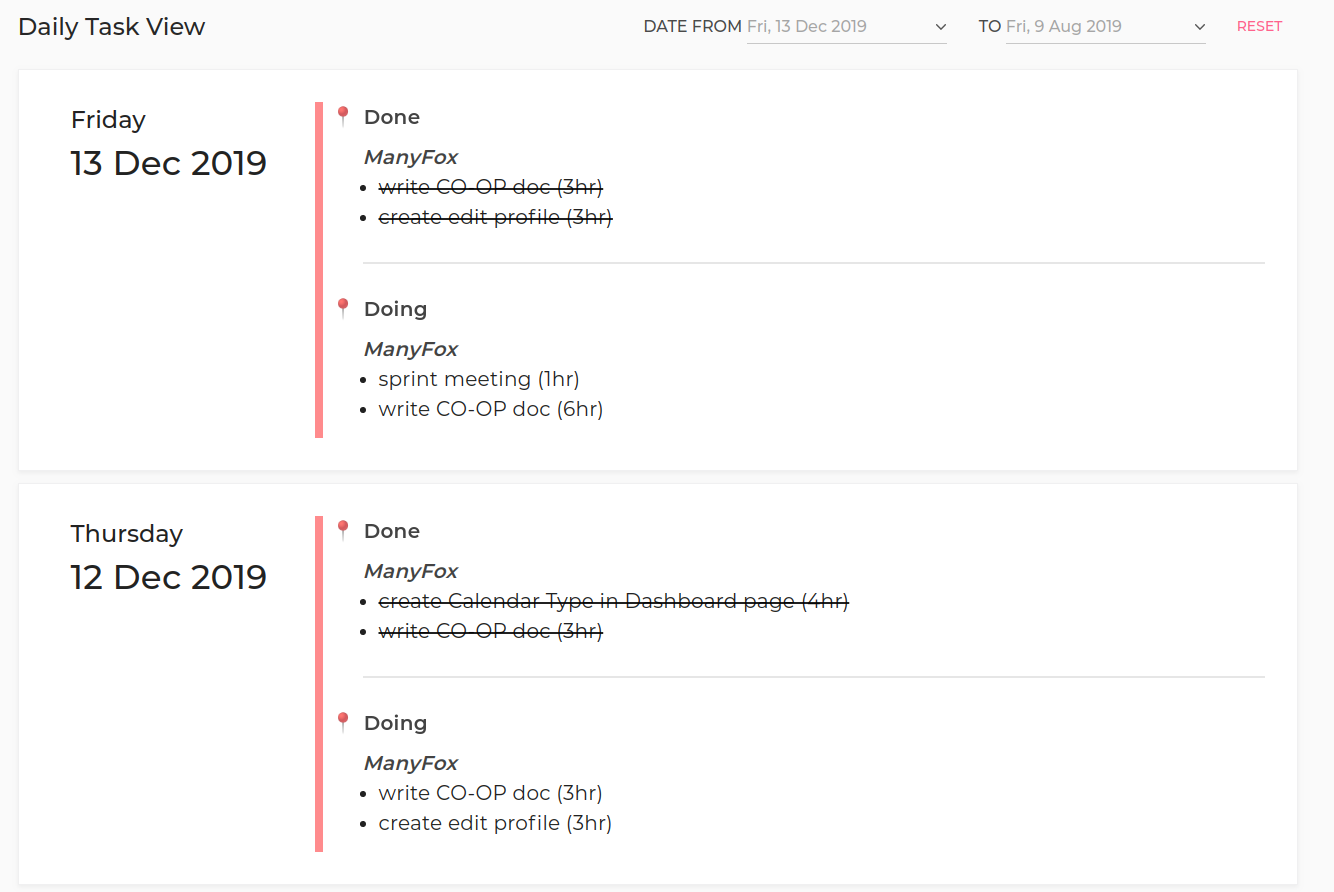
\includegraphics[width=1\linewidth]{daily-task-1}
	\caption{Daily task}
	\label{Fig:daily-task-1}
\end{figure}
\vskip1em หากมีการลาในวันนั้น จะแสดงข้อมูล เหตุผลการลา ระยะเวลาการลา และประเภทการลา ด้านซ้ายมือของของ กล่อง daily task


\vskip1em หากไม่ได้เขียน daily task ในวันนั้น กล่อง daily task จะเป็นสีชมพูและ มีข้อความ You don\'t write a task ขึ้น

\vskip1em โดยในหน้า Daily task ใช้วิธี Pagination แบบ Cursor Pagination โดยการ Query ครั้งแรกจะได้ข้อมูล 10วันล่าสุดและเมื่อเลื่อนหน้าจอถึงด้านล่างสุดจะ
Query ข้อมูล 10วันถัดมาโดยใช้การส่ง Id จะข้อมูลdaily task ท้ายสุดในการหาข้อมูลถัดมา และสามารถ filter เลือกเฉพาะช่วงวันที่ต้องการได้
\subsection{Search users}
component Search user จะสามารถใช้งานได้เฉพาะผู้มี permission "see\_report" เท่านั้น โดยจะสัญลักษณ์ แว่นขยาย อยู่ด้านขวาบนเมื่อคลิ๊กที่สัญลักษณ์จะมีกล่องค้นหา user สไลด์ออกมาและ เริ่ม Query ข้อมูลของ user ทั้งหมดภายใน workspaceนั้น
เมื่อพิมพ์ข้อความ จะปรากฎรายชื่อ user ประกอบด้วยรูป user ชื่อ และวันลาที่เหลือ โดยค้นหาตามชื่อของ user ที่ประกอบข้อความที่พิมพ์
เมื่อกดที่ user คนใดคนหนึ่ง กล่องจะสไลด์กลับและเปลี่ยนไปหน้า Individual Report ของ user นั้น
\begin{figure}[!htbp]
	\centering
	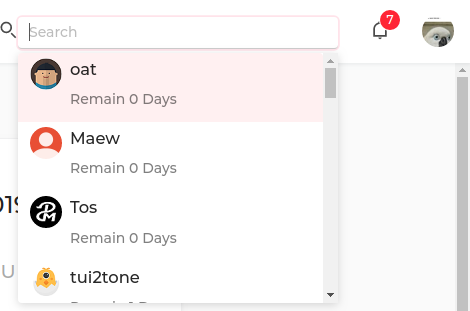
\includegraphics[width=0.4\linewidth]{search-users}
	\caption{Search users}
	\label{Fig:search-users}
\end{figure}


\subsection{Notifications}
component Notifications เป็นสัญลักษณ์กระดิ่ง และจะมีตัวเลขจำนวนการแจ้งเตือนที่ไม่ได้อ่านอยู่ด้านบนขวาของกระดิ่ง มีตำแหน่งอยู่ที่ด้านบนขวาของหน้าถัดจาก Search user และเมื่อกดคลิ๊กที่กระดิ่ง
จะมีรายการข้อความแจ้งเตือนต่างๆ โดยข้อความที่ยังไม่อ่านจะมีพิ้นหลังสีเทา และข้อความที่อ่านแล้วจะมีพื้นหลังสีขาว
เมื่อกดที่ข้อความนั้นจะเด้งไปหน้าที่เลือกไว้ และเปลี่ยนสถานะเป็นอ่านแล้ว หรือ กดปุ่มด้านบนขวาของรายการ "MARK ALL AS READ" เมื่อกดแล้ว จะเปลี่ยนสถานะข้อความทั้งหมดเป็นอ่านแล้ว

\begin{figure}[!htbp]
	\centering
	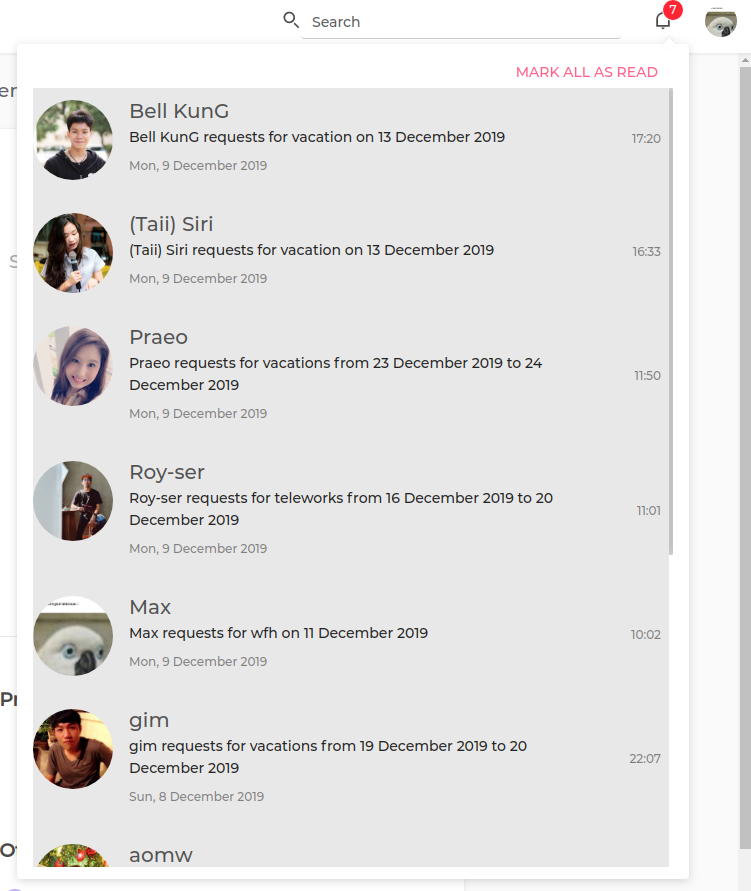
\includegraphics[width=0.5\linewidth]{notifications}
	\caption{Notifications}
	\label{Fig:notifications}
\end{figure}

\subsection{Dashboard}
หน้า Dashboard เป็นหน้าสำหรับ ผู้มี permission approve\_request และ add\_calendar ถึงสามารถเข้าใช้งานได้
โดยประกอบไปด้วย 3 component และ 2 Modal ดังนี้
\subsubsection{Request Offworks}
เป็น component แสดงรายการคำร้องขอลางาน จะแสดงข้อมูลการลา รูปโปรไฟล์ ชื่อ ตำแหน่ง ประเภทการลา เหตุผลการลา ระยะเวลาการลา และวันที่ลา ขอพนักงานผู้เขียนคำร้อง
และมีปุ่ม Approve และ X อยู่ด้านขวามือ เมื่อกดปุ่ม Approve หมายถึงยืนยันการลา และส่งแจ้งเตือนไปยังพนักงานผู้เขียนคำร้องทั้งใน เว็บไซต์และ slack
เมื่อกดปุ่ม X จะมีกล่อง Modal ให้กรอกเหตุผลการปฎิเสธการลางาน เมื่อกด submit จะส่งแจ้งเตือนพร้อมเหตุผลไปยังพนักงานผู้เขียนคำร้องทั้งใน เว็บไซต์และ slack
และสามารถคัดกรองร้องผ่านช่วงเวลา (ทั้งหมด ภายในอาทิตย์นี้ ถายในเดือนนี้ และ ภายในปีนี้) หรือคัดกรองผ่านตำแหน่งได้
\begin{figure}[!htbp]
	\centering
	\subfigure[Request Offwork list]{
		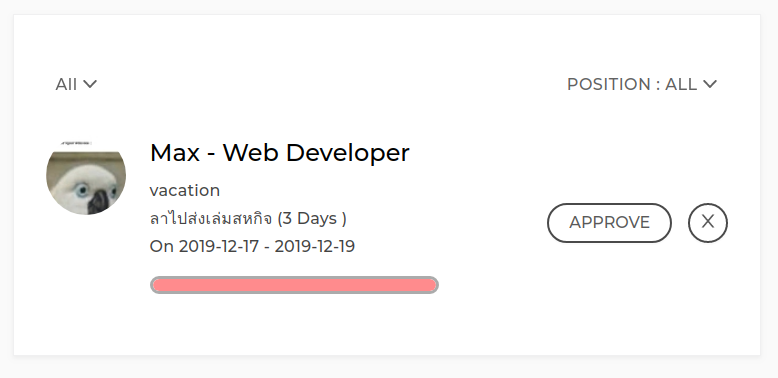
\includegraphics[width=0.8\linewidth]{request-offwork}
		\label{Fig:request-offwork-list}
	}
	\subfigure[Reject modal]{
		\label{Fig:reject-modal}
		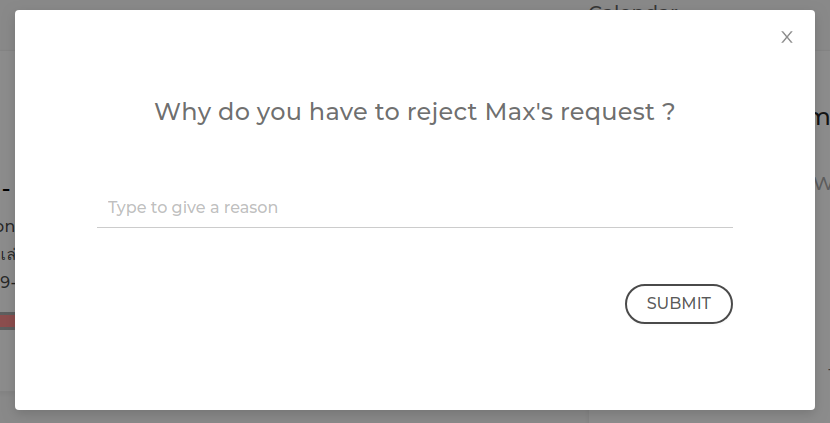
\includegraphics[width=0.8\linewidth]{reject-modal}
	}
	\caption{Request Offwork}
	\label{Fig:request-offwork}
\end{figure}
\subsubsection{Overall Summary Report}
เป็น component แสดง Area Graph การลางานของพนักงานทั้งหมดภายในปีนี้ แบ่งประเภทการลาตามสี
และสามารถ Export ข้อมูลออกมาผ่านปุ่ม \textbf{Export} ด้านขวาบน เมื่อกดจะดาวโหลดไฟล์ Excel ข้อมูลการลามาในรูปแบบตาราง โดยจะส่งมาตามช่วงที่เลือกไว้
โดยสามารถเลือกรูปแบบได้ 3 รูปแบบดังนี้
\vskip1em รูปแบบ \textbf{Year} จะแสดงเป็นกราฟโดยแบ่งออกเป็น 12 ช่วงตามเดือน
\begin{figure}[!htbp]
	\centering
	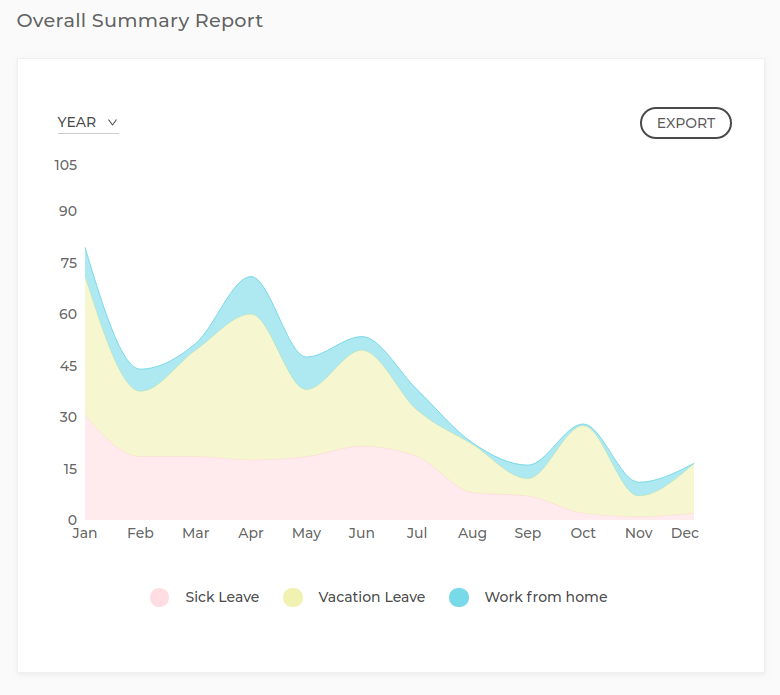
\includegraphics[width=0.5\linewidth]{graph-report-1}
	\caption{Overall Summary Report รูปแบบ Year}
	\label{Fig:graph-report-1}
\end{figure}
\vskip1em รูปแบบ \textbf{Month} จะมีเมนูให้เลือกเดือนและแสดงกราฟโดยแบ่งออกตามวันภายในเดือนนั้น
\begin{figure}[!htbp]
	\centering
	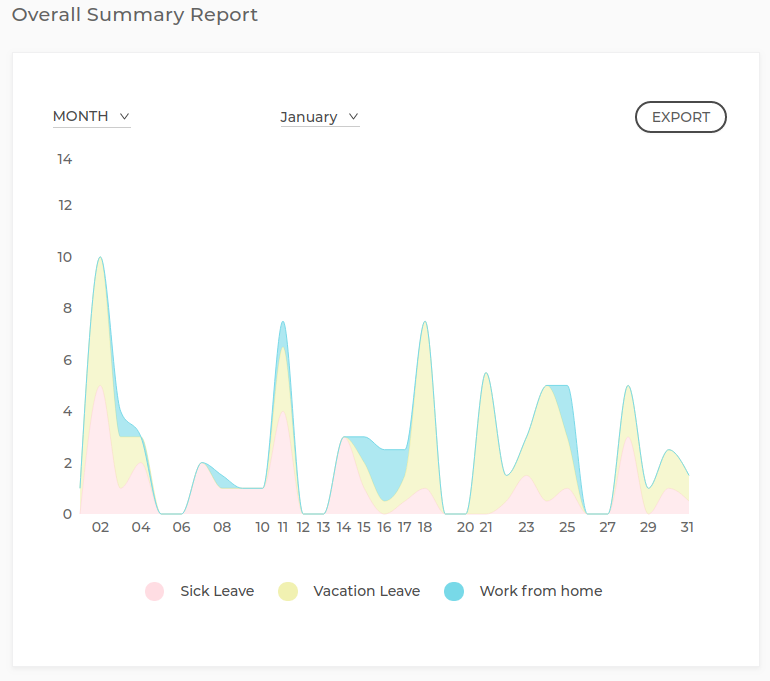
\includegraphics[width=0.5\linewidth]{graph-report-2}
	\caption{Overall Summary Report รูปแบบ Month}
	\label{Fig:graph-report-2}
\end{figure}
\vskip1em รูปแบบ \textbf{Custom}  จะมีเมนูเลือกเดือนที่เริ่มต้น จนถึงเดือนที่ต้องการและแสดงกราฟโดยแบ่งตามวันภายในช่วงที่เลือก
\begin{figure}[!htbp]
	\centering
	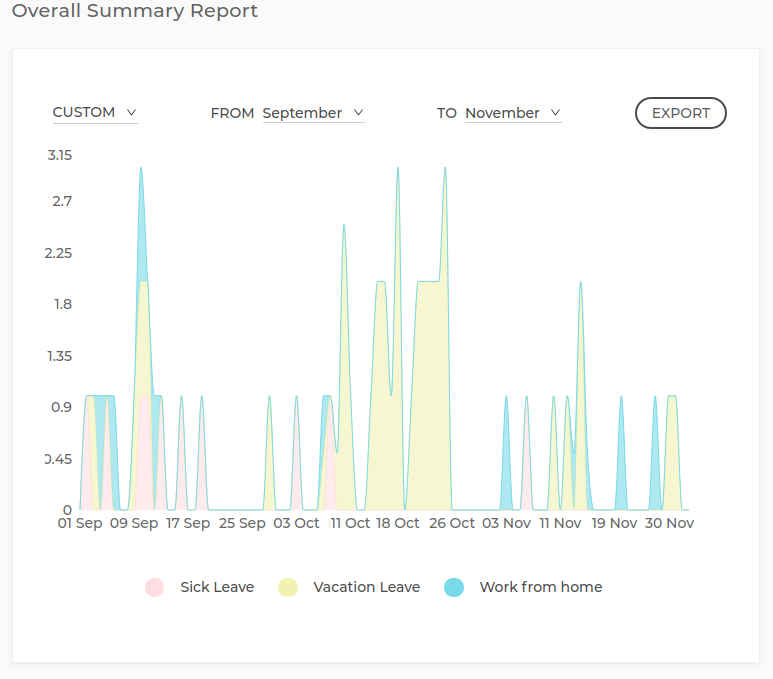
\includegraphics[width=0.7\linewidth]{graph-report-3}
	\caption{Overall Summary Report รูปแบบ Custom}
	\label{Fig:graph-report-3}
\end{figure}
\subsubsection{Calendar Controller}
เป็น component ไว้สำหรับสร้าง และลบ Event ภายใน Calendar โดยแบ่งเป็นอีก 2 ส่วนคือ Calendar และ Calendar Type
โดยส่วนของ Calendar เมื่อกดที่วันที่จะแสดง Calendar Modal ขึ้นมา
\vskip1em \textbf{Calendar Type} จะแสดงประเภทและสีของ Calendar และสามารถ สร้าง แก้ไขและลบชื่อหรือสีของ Calendar Type ได้
\newpage
\begin{figure}[!htbp]
	\centering
	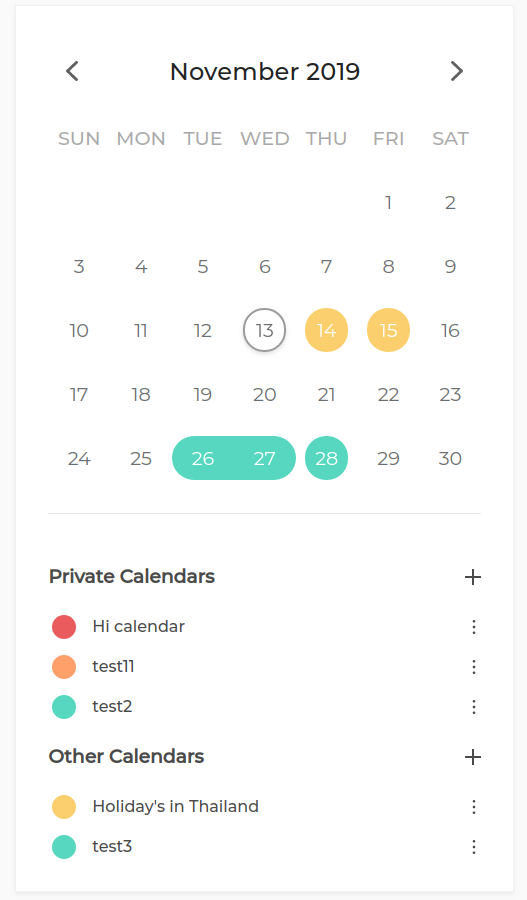
\includegraphics[width=0.5\linewidth]{calendar-controller}
	\caption{Calendar Controller}
	\label{Fig:calendar-controller}
\end{figure}

\subsubsection{Calendar Modal}
กล่อง Calendar Modal หลังจากกดวันที่ใน Calendar มีไว้เพื่อ แสดงข้อมูล Event ณ วันที่กด หากไม่มี Event ใันวันนั้นจะมีปุ่ม + เมื่อกดจะเปลี่ยนเป็นกล่องสำหรับกรอกข้อมูลสร้าง Event โดยประกอบด้วย
ชื่อหัวข้อ Event  วันที่เริ่ม-วันสุดท้าย Event และ Calendar Type เมื่อกดปุ่ม ADD จะบันทึกข้อมูลลง Database และปิด Modal พร้อม update Query ใน component Calendar
\newpage
\begin{figure}[!htbp]
	\centering
	\subfigure[no Event]{
		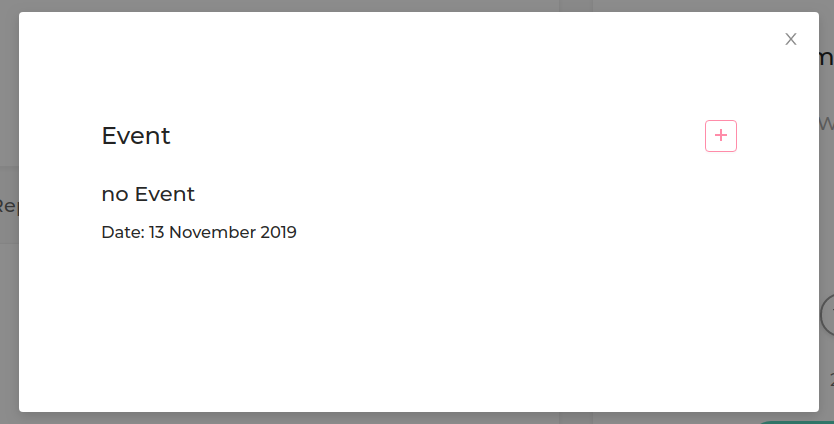
\includegraphics[width=0.75\linewidth]{calendar-modal-1}
		\label{Fig:calendar-modal-1}
	}
	\subfigure[Event]{
		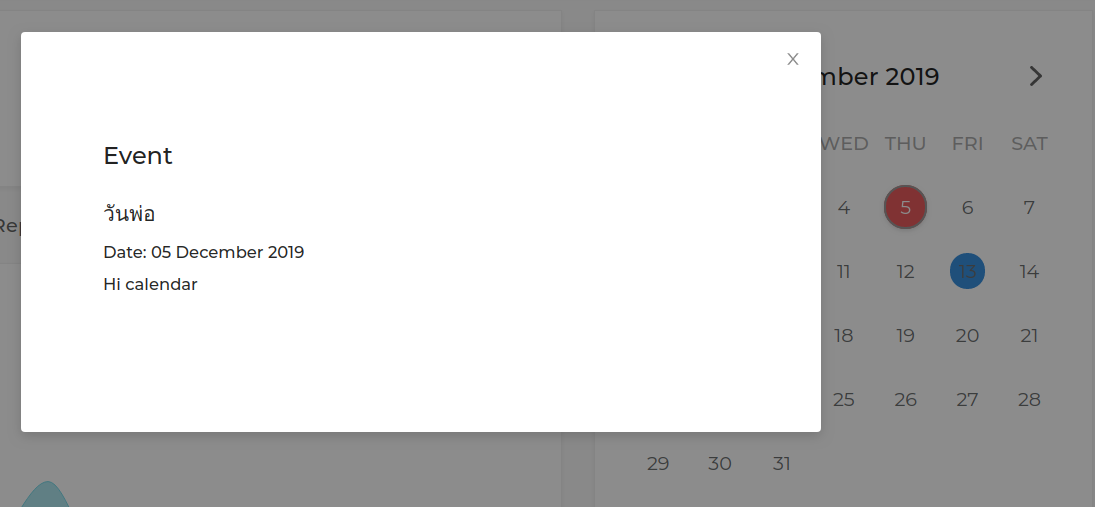
\includegraphics[width=0.75\linewidth]{calendar-modal-2}
		\label{Fig:calendar-modal-2}
	}
	\subfigure[ADD Event]{
		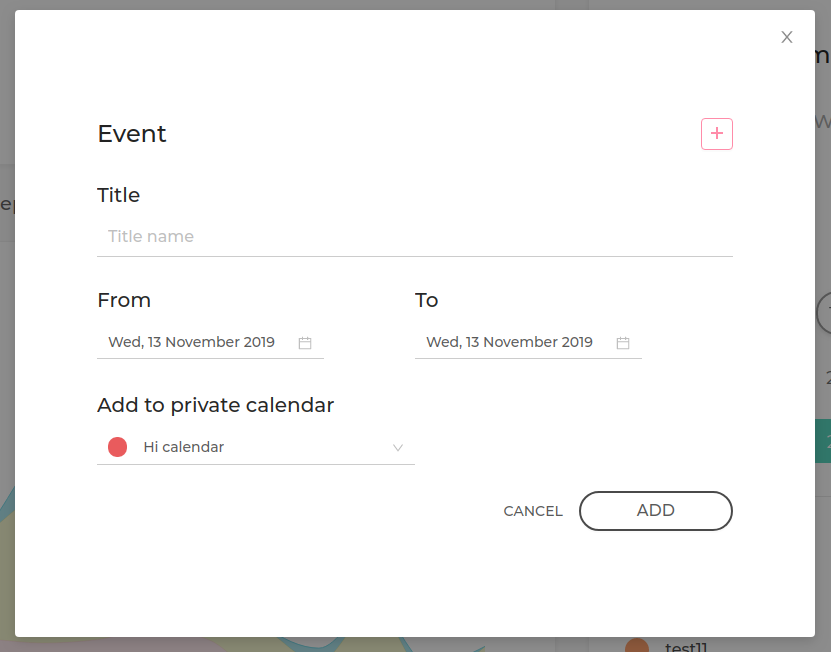
\includegraphics[width=0.75\linewidth]{calendar-modal-3}
		\label{Fig:calendar-modal-3}
	}
	\caption{Calendar Modal}includegraphics

\end{figure}
\subsubsection{Calendar Type Modal}
กล่อง Modal สำหรับการเพิ่ม แก้ไข หรือลบ Calendar Type และสามารถกด เปิดหรือปิด Calendar Type นั้นๆ
โดยจะส่งผลให้ข้อมูลCalendar ที่มี Calendar Type ที่ถูกปิดจะถูกซ่อนใน Calendar ไปด้วย
\subsection{Leave Setting}
Leave Setting เป็นหนึ่งในหน้าย่อยของ Workspace Setting เป็นส่วนตั้งค่าเกี่ยวกับการลาของพนักงานโดยจะแบ่งตาม
รูปแบบการจ้างงาน (Employment)โดยสามารถตั้งค่าประเภทการลาได้ดังนี้
\vskip1em \textbf{ลาพักร้อน (Vacation Leave)} สามารถตั้งจำนวนวันลาพักร้อนภายใน1ปี (โดยระบบจะทยอยเพิ่มในวันที่1 ของเดือนถัดไป)
และสามารถตั้งให้สามารถลาได้เฉพาะในอาทิตย์ถัดไป(นับจากวันศุกร์ขึ้นไป ถือว่าเริ่มอาทิตย์ใหม่)
\vskip1em \textbf{ลาป่วย (Sick Leave) }นั้นจะเป็นรูปแบบอนุมัติการลาอัตโนมัติ โดยสามารถตั้งค่าลาป่วยติดต่อกี่วัน ถึงจำเป็นต้องได้รับการอนุมัติ
\vskip1em \textbf{ทำงานที่บ้าน (Work form home)} สามารถตั้งจำนวนวันทำงานที่บ้านมากที่สุดต่อ 1 อาทิตย์
และสามารถตั้งให้สามารถลาได้เฉพาะในอาทิตย์ถัดไป(นับจากวันศุกร์ขึ้นไป ถือว่าเริ่มอาทิตย์ใหม่)
\vskip1em \textbf{ทำงานต่างสาขา (Work from other Branch)} สามารถตั้งให้สามารถลาได้เฉพาะในอาทิตย์ถัดไป(นับจากวันศุกร์ขึ้นไป ถือว่าเริ่มอาทิตย์ใหม่)
\vskip1em \textbf{ลาไปอบรม (seminar Leave)} สามารถตั้งให้สามารถลาได้เฉพาะในอาทิตย์ถัดไป(นับจากวันศุกร์ขึ้นไป ถือว่าเริ่มอาทิตย์ใหม่)

\subsection{Bot Setting}
Bot Setting เป็นหนึ่งในหน้าย่อยของ Workspace Setting เป็นหน้าควบคุมตั้งค่าที่เกี่ยวข้องกับ Slack bot
โดยแบ่งเป็น 3 หน้าดังต่อไปนี้
\subsubsection{Who off works}
หน้าตั้งค่าการแสดงข้อมูลบุคคลที่ลาและข้อมูลการลาภายใน Slack โดยหากเลื่อน Switch ด้านขวาเป็น ON
จะแจ้งเตือนข้อมูลบุคคลที่ลาและข้อมูลการลา ตามเวลาที่กำหนดของทุกวันที่ทำงานและสามารถแก้ไขข้อความด้านใต้ของข้อมูลบุคคลที่ลาและข้อมูลการลาได้
และกำหนดChannel ที่ต้องการให้แสดงผล และสามารถใช้งาน /whooffworks และ /offwork command ภายใน Channel นั้นได้
\subsubsection{Auto-reply}
หน้าตั้งค่าการคำตอบสนองอัตโนมัติจาก Manyfox bot ภายใน Slack โดยสามารถเพิ่ม ลบหรือแก้ไข คำตอบสนองได้มากถึง 50 รูปแบบ โดยแต่ละรูปแบบประกอบไปด้วย
Keyword ที่ต้องการตรวจจับโดยเพิ่มได้มากสุด 5 คำ และ Response คำตอบที่เมื่อจับ1ในคำที่อยู่ Keyword จะแสดงผลคำตอบ (มากสุด 50 ตัวอักษร) โดยหากมีมากกว่า 1 จะสุ่มคำตอบ โดยสามารถเลือก Channel ที่ต้องการสามารถใช้ Auto-reply ได้มากกว่า 1
หรือสามารถเลือก All Channel เพื่อต้องการให้ใช้งานได้ในทุก Channel
\subsubsection{Daily task}
หน้าตั้งค่าการแสดงการเขียน Daily task ภายใน Slack โดยหากเลื่อน Switch ด้านขวาเป็น ON
จะแจ้งเตือนข้อความรายชื่อบุคคลที่ไม่เขียน task ภายในวันนี้ โดยใช้วิธีการแท๊ก ทำให้จะขึ้นแจ้งเตือนแม้ว่าจะปิดการแจ้งเตือนไว้ก็ตาม
โดยจะแสดงตามเวลาที่กำหนดของทุกวันที่ทำงาน และสามารถแก้ไขข้อความด้านใต้ของรายชื่อได้
\vskip1em กล่องขวาจะมีส่วนกำหนด Channel ที่ต้องการให้แสดงผล และสามารถใช้งาน /task command ภายใน Channel นั้นได้
และมีส่วนสำหรับการกำหนด บุคคลที่จะเป็น Whitelist และ Watcher โดย Whitelist หมายถึง บุคคลที่ไม่ได้เขียน task แต่จะไม่ถูกแท็กและมีรายชื่อในแจ้งเตือน (เช่น กรณี ผู้บริหารที่ไม่จำเป็นต้องการโดนแท็ก)
และ Watcher หมายถึงบุคคลที่แม้ว่าจะเขียน task แล้ว ก็ยังถูกแท็กและขึ้นแจ้งเตือน (เช่น กรณี ผู้บริหารที่ต้องการโดนแท็ก เพื่อดูความคืบหน้าพนักงาน)

\begin{figure}[!htbp]
	\centering
	\subfigure[Who off works]{
		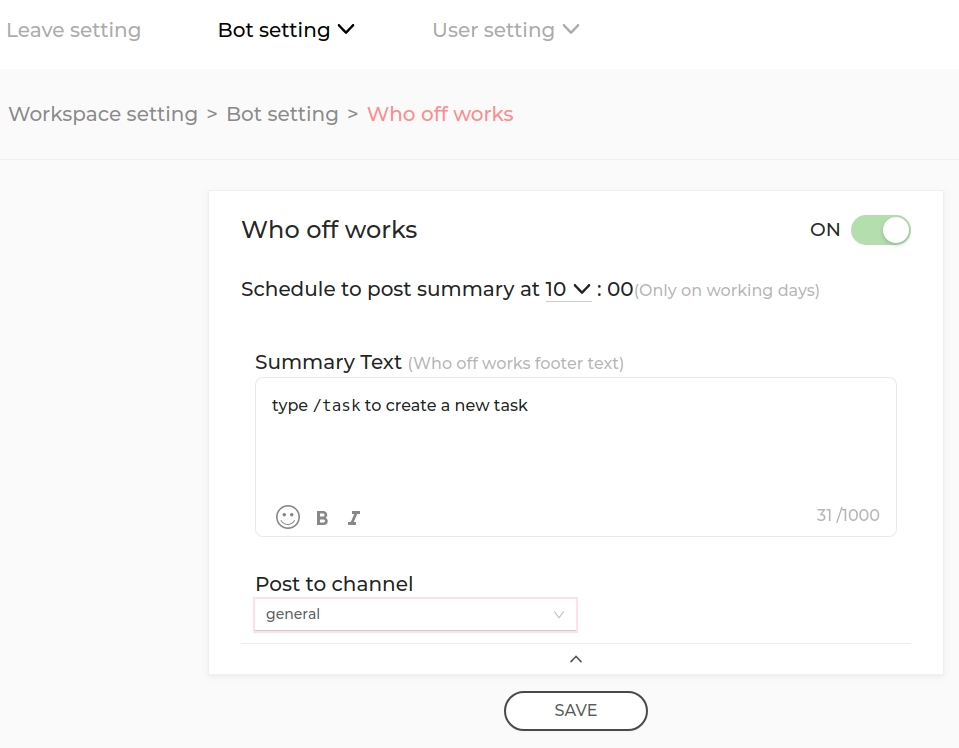
\includegraphics[width=0.48\linewidth]{bot-setting-1}
		\label{Fig:bot-setting-1}
	}
	\subfigure[Auto-reply]{
		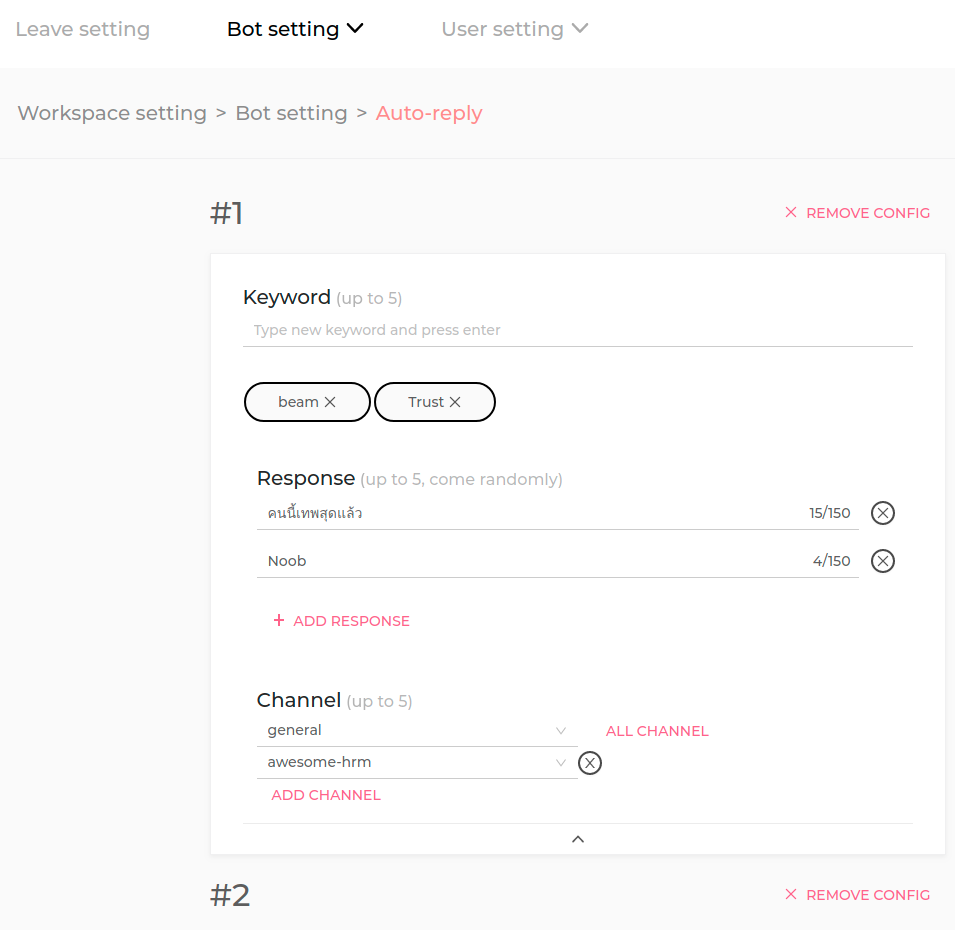
\includegraphics[width=0.48\linewidth]{bot-setting-3}
		\label{Fig:bot-setting-3}
	}
\end{figure}
\begin{figure}[!htbp]
	\centering
	\subfigure[Daily task]{
		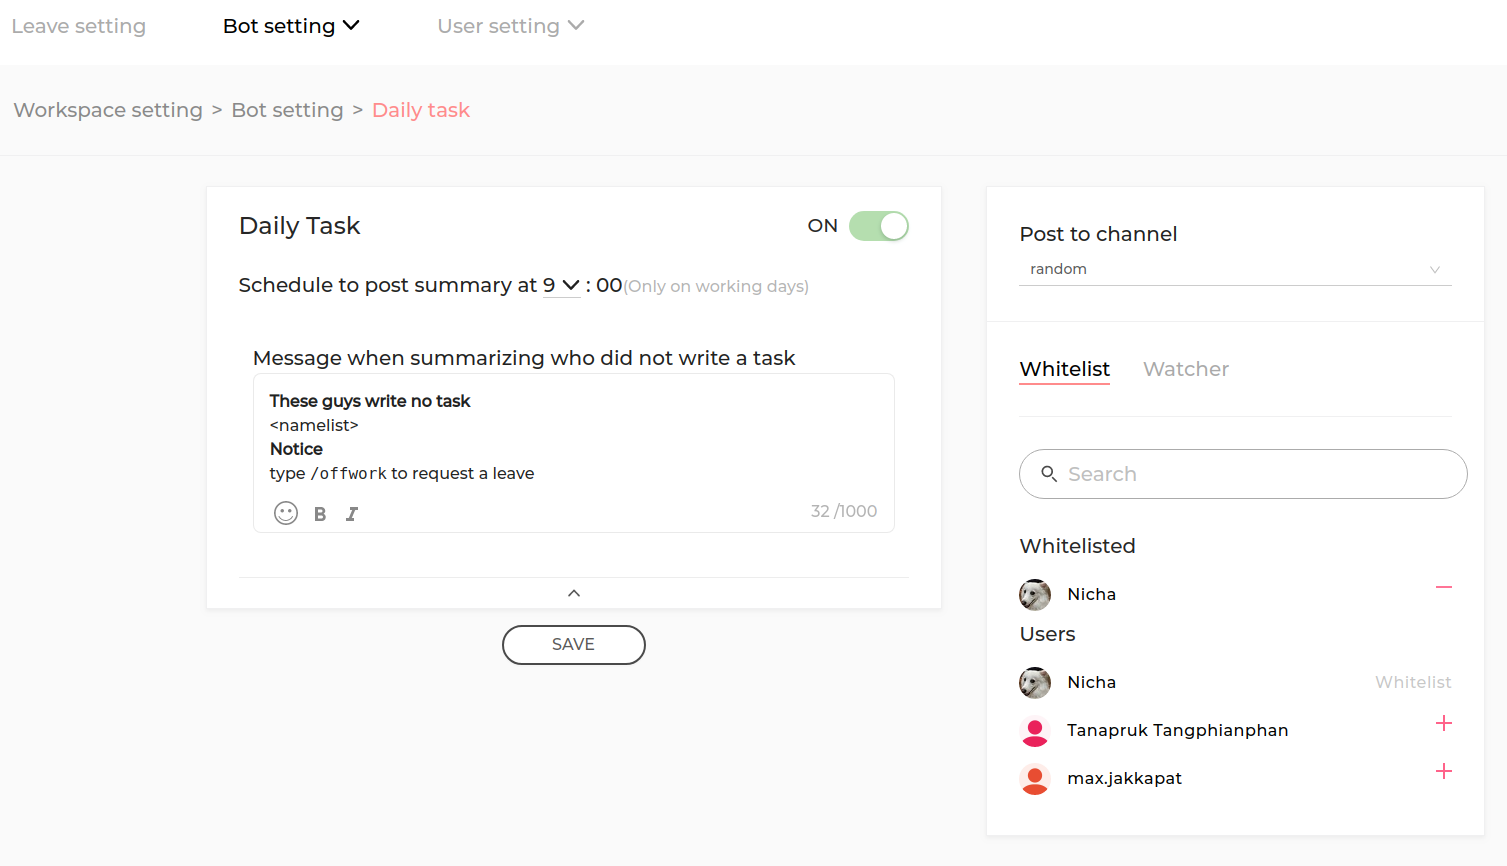
\includegraphics[width=0.75\linewidth]{bot-setting-2}
		\label{Fig:bot-setting-2}
	}
	\caption{Bot Setting}
\end{figure}
\subsection{User Setting}
User Setting เป็นหนึ่งในหน้าย่อยของ Workspace Setting เป็นหน้าควบคุมตั้งค่าที่เกี่ยวกับสถานะของ ตำแหน่ง ระดับชั้น และรูปแบบการจ้างงานโดยแบ่งเป็น 3 หน้าดังต่อไปนี้
\subsubsection{Employment}
Employment หรือ รูปแบบการจ้างงาน เป็นหน้าควบคุมตั้งค่าสำหรับ เพิ่ม ลบ และแก้ไข รูปบบการจ้างงาน
\subsubsection{Level}
Level หรือ ลำดับชั้น เป็นหน้าควบคุมตั้งค่าสำหรับ เพิ่ม ลบ และแก้ไข ลำดับชั้นภายในบริษัท และสามารถตั้งค่าจำกัดการเข้าถึงข้อมูลในแต่ละได้ตามลำดับชั้น
\subsubsection{Job Title}
Job Title หรือ ตำแหน่ง เป็นหน้าควบคุมตั้งค่าสำหรับ เพิ่ม ลบ และแก้ไข ตำแหน่งหน้าที่ภายในบริษัท
\subsection{Master Calendar Setting}
หน้าสำหรับตั้งค่า ของ Manyfox Administrator เท่านั้น สำหรับการเพิ่ม ลบ หรือแก้ไข Public Calendar
\subsection{Feedback}
หน้า Feedback เป็นหน้าสำหรับ แสดงคำถามพบบ่อย (FAQ) และรับฟังความเห็นหรือแจ้งปัญหาของแอพพลิเคชั่น โดยด้านซ้ายจะเป็น FAQ
เมื่อกดที่กล่องหัวข้อคำถาม จะมีข้อความรายะละเอียดโผล่มาด้านล่างของหัวข้อ ส่วนด้านขวาจะเป็นแบบฟอร์มรับฟังความเห็น หรือแจ้งปัญหาโดยต้องกรอก หัวข้อ ข้อความแสดงความคิดเห็น และอีเมลติดต่อกลับ
และสามารถอัพโหลดรูปภาพได้มากถึง 5 รูป โดยแต่ละรูปมีขนาดไม่เกิน 2MB เมื่อกด Submit จะส่งแบบฟอร์มไปเก็บบน Database และมี mail ตอบรับเข้าไปยัง Emailที่กรอกไป

\begin{figure}[!ht]
	\centering
	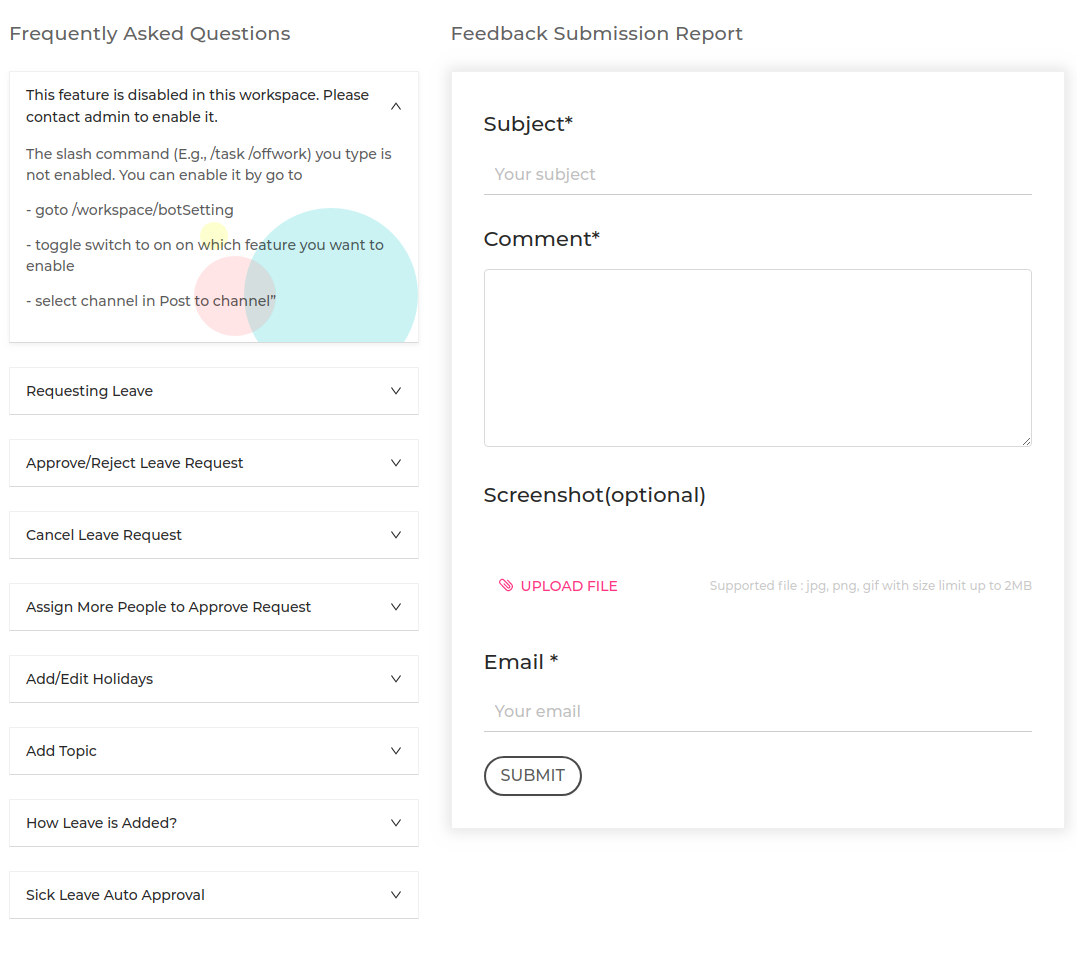
\includegraphics[width=0.8\linewidth]{feedback}
	\caption{Feedback}
	\label{Fig:feedback}
\end{figure}

\subsection{/offwork command}
เมือเรียกใช้คำสั่ง \textbf{/offwork} บนกล่องแชทใน channel ของ Slack ที่กำหนดในหน้า bot setting ในหัวข้อ Who off works จะปรากฎกล่องแบบฟอร์มสำหรับเขียนคำร้องลางาน โดยมีช่องสำหรับเลือกประเภทการลา ระยะเวลาการลา
เหตุผลการลา วันที่ลา และวันสุดท้ายที่ลา (กรณีลามากกว่า 1 วัน) เมื่อกด submit จะส่งข้อมูลไปเก็บบน Database และมีข้อความรายละเอียดการลาขึ้นในห้องแชท channel ที่เลือก
\begin{figure}[!ht]
	\centering
	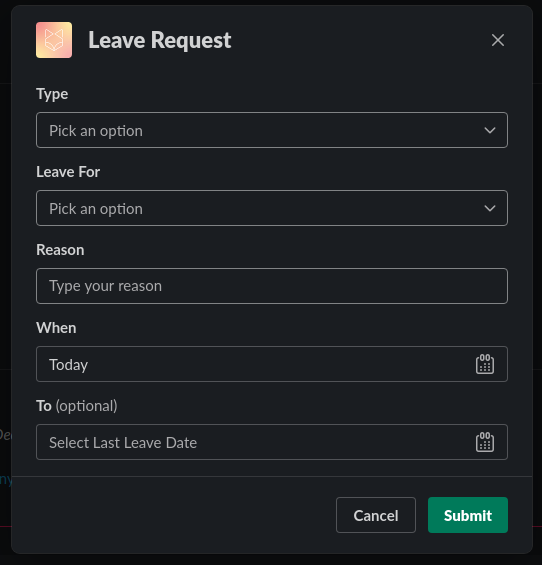
\includegraphics[width=0.6\linewidth]{offwork-command}
	\caption{/offwork-command}
	\label{Fig:offwork-command}
\end{figure}
\subsection{/whooffworks command}
เมื่อเรียกใช้คำสั่ง \textbf{/whooffworks} บนกล่องแชทใน channel ของ Slack ที่กำหนดในหน้า bot setting
ในหัวข้อ Who off works จะปรากฎข้อมูลบุคคลที่ลาและข้อมูลการลา ของวันนี้ขึ้นบนห้องแชทใน channel นั้น
\vskip1em และหาก ใช้คำสั่ง \textbf{/whooffworks tmr} จะขึ้นข้อมูลการลาของวันพรุ่งนี้แทน
\begin{figure}[!htbp]
	\centering
	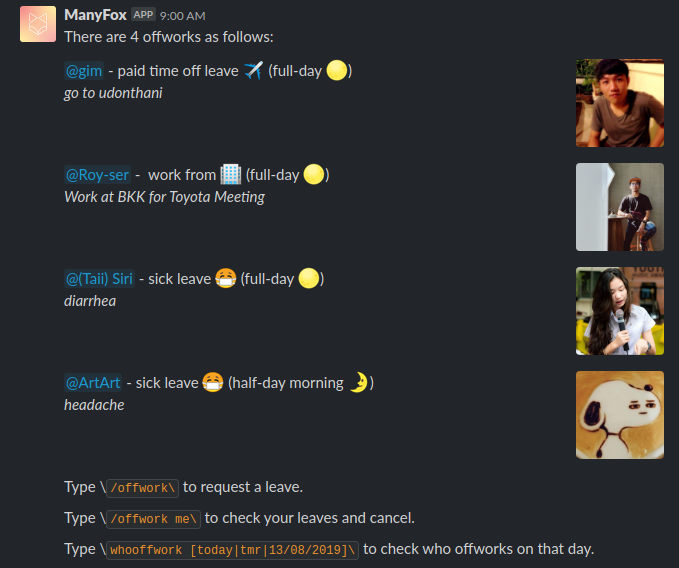
\includegraphics[width=0.6\linewidth]{whooffwork-command}
	\caption{/whooffwork-command}
	\label{Fig:whooffwork-command}
\end{figure}
\subsection{/task command}
เมื่อเรียกใช้คำสั่ง \textbf{/task} บนกล่องแชทใน channel ของ Slack ที่กำหนดในหน้า bot setting ในหัวข้อ Daily task จะปรากฎกล่องแบบฟอร์มสำหรับ การเขียน task
โดยวิธีเขียน task คือเขียน 1 task ต่อ 1 บรรทัด และต้องลงท้ายด้วย ระยเวลาชมที่ใช้ เช่น
\\\textbf{เขียนรายงานสหกิจ (7.5hr)}
และแบ่งช่องในการเขียน daily task เป็น 4 ส่วนดังนี้
\\\textbf{DONE} เขียน task ที่ทำเสร็จของวันที่แล้ว จำเป็นต้องเขียน
\\\textbf{DOING} เขียน task ที่จะทำในวันนี้ จำเป็นต้องเขียน
\\\textbf{TODO} เขียน task สิ่งต้องทำในวันข้างหน้า
\\\textbf{Note} เขียน ข้อความเตือนความจำตนเอง
\vskip1em เมื่อกด Submit จะเก็บข้อมูลบน Database และขึ้นข้อมูล task ที่เขียนไปบนห้องแชท channel ที่เลือก
\vskip1em หากใช้คำสั่ง \textbf{/task me} จะขึ้นข้อมูล task ของผู้ใช้ที่เขียนล่าสุดใน ห้องแชท โดยข้อความนั้นจะมีเพียงผู้ใช้ที่เห็น
\vskip1em หากใช้คำสั่ง \textbf{/task edit} จะขึ้นกล่องแบบฟอร์มในการแก้ไข้ task ล่าสุดที่เขียนไป โดยจะมี task เดิมอยู่บนช่องกรอกข้อมูลไว้แล้ว
เมื่อ submit จะเป็นการบันทึกทับข้อมูล task ของเก่า และขึ้นข้อมูล task ล่าสุดบนห้องแชทอีกรอบ
\begin{figure}[!htbp]
	\centering
	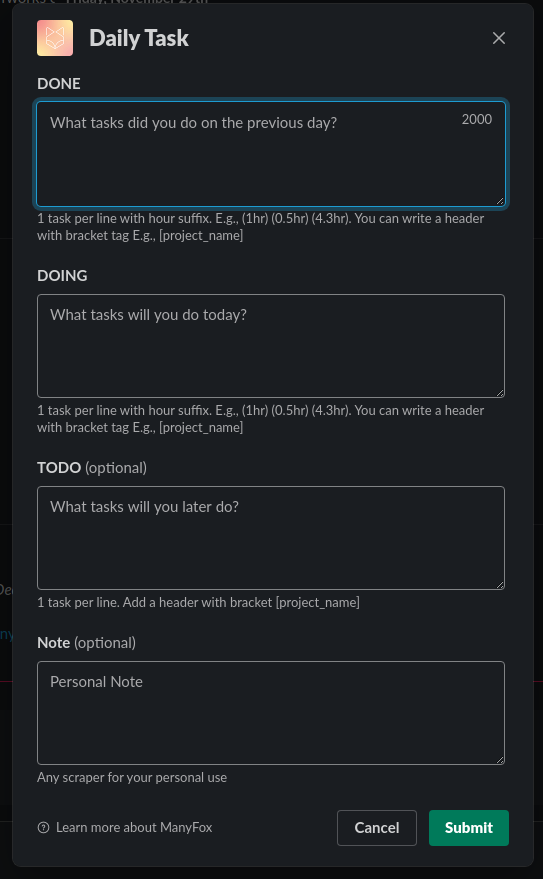
\includegraphics[width=0.4\linewidth]{task-command}
	\caption{/task-command}
	\label{Fig:task-command}
\end{figure}
\subsection{/meeting command}
เมือเรียกใช้คำสั่ง \textbf{/meeting} บทกล่องแชท จะปรากฎกล่องแบบฟอร์มสำหรับการนัดประชุม
โดยต้องกรอกหัวข้อประชุม รายละเอียดการประชุม วันที่ประชุม เวลาเริ่มต้นประชุม ระยะเวลาการประชุม สถานที่จัดประชุม และผู้เข้าร่วมประชุม
เมื่อกด Create จะขึ้นข้อมูลการนัดประชุม และแท๊กและแจ้งเตือนไปยังบุคคลที่นัดประชุมใน slack
\begin{figure}[!htbp]
	\centering
	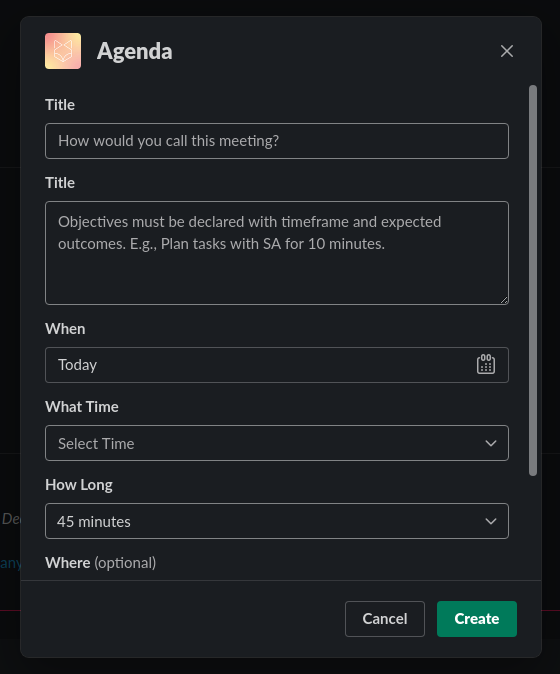
\includegraphics[width=0.8\linewidth]{meeting-command-1}
	\caption{/meeting-command-1}
	\label{Fig:meeting-command-1}
\end{figure}
\subsection{Auto increase remain offwork}
เมื่อถึงวันที่ 1 ของทุกเดือนระบบจะทำการเพิ่มวันที่จำนวนวันลาพักร้อนที่เหลือ ตามจำนวนที่บริษัทกำหนด และตามประเภทการจ้างงาน
\subsection{Landing page}
หน้าเว็บไซต์สำหรับนำเสนอ Manyfox โดยกล่าวถึงรายละเอียด Feature ต่างๆ
\begin{figure}[!htbp]
	\centering
	

\end{figure}
\begin{figure}[!htbp]
	\centering
	\subfigure[Section-1]{
		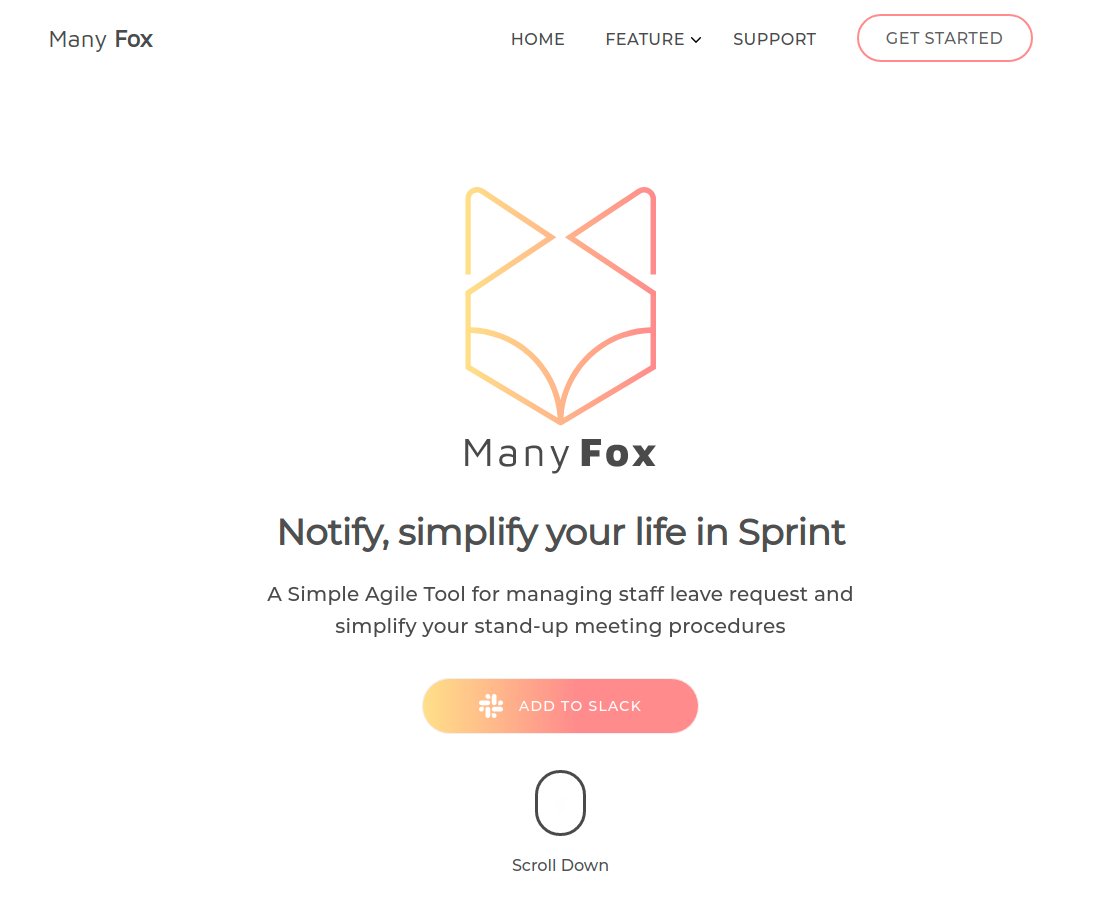
\includegraphics[width=0.7\linewidth]{landing-page-1}
		\label{Fig:landing-page-1}
	}
	\subfigure[Section-2]{
		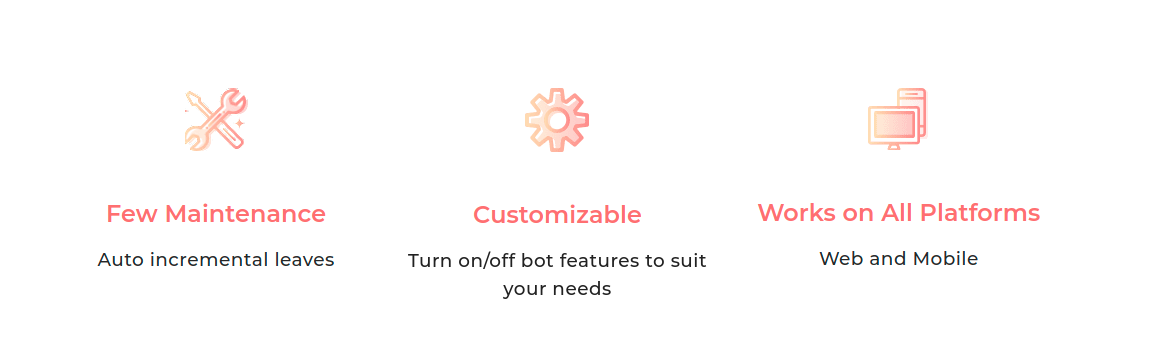
\includegraphics[width=0.7\linewidth]{landing-page-2}
		\label{Fig:landing-page-2}
	}
	\subfigure[Sectio-3]{
		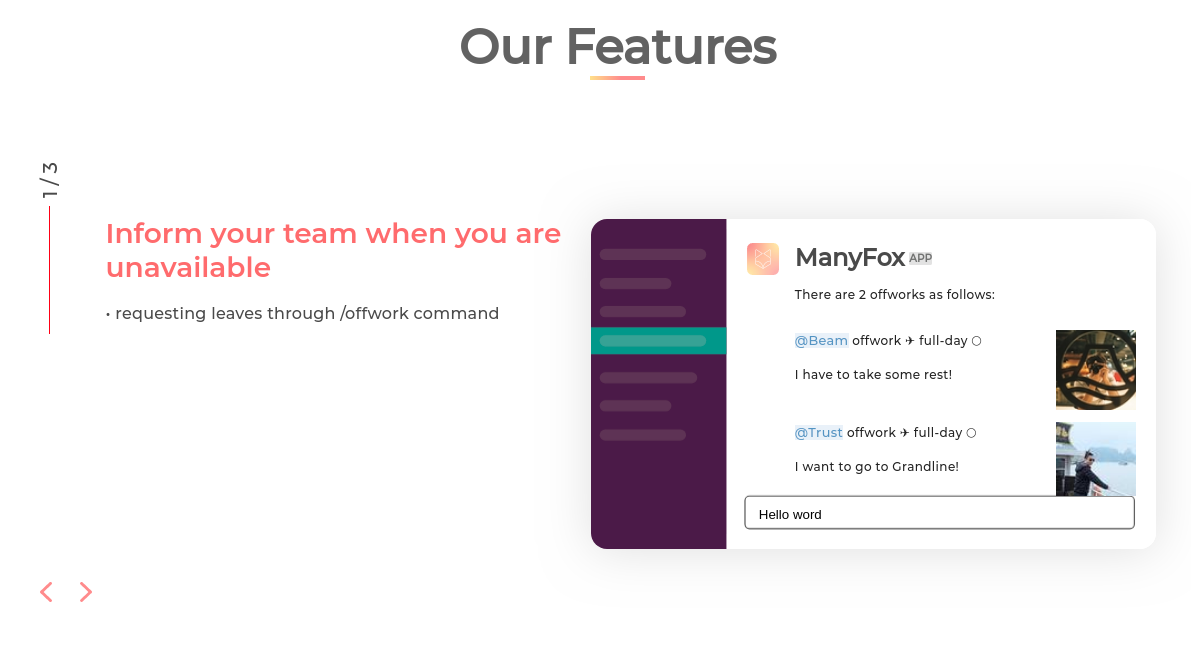
\includegraphics[width=0.7\linewidth]{landing-page-3}
		\label{Fig:landing-page-3}
	}
\end{figure}

\begin{figure}[!htbp]
	\centering
	\subfigure[Section-4]{
		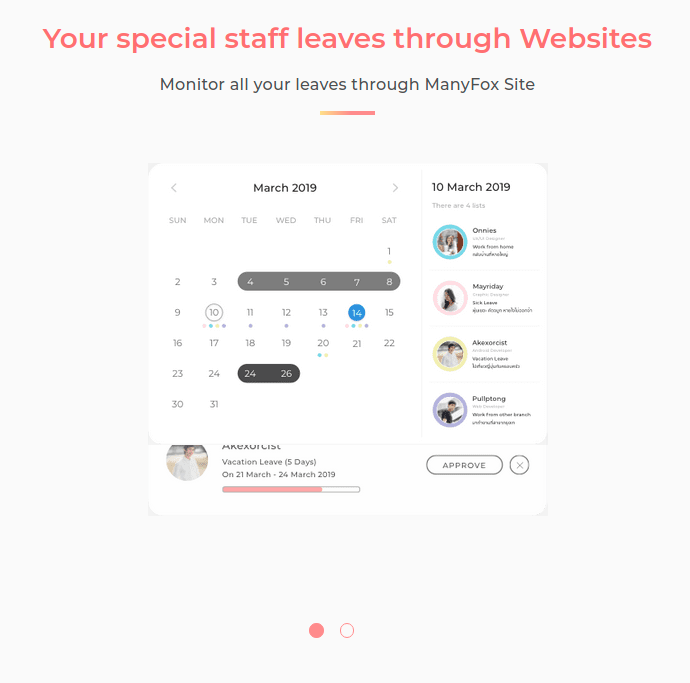
\includegraphics[width=0.5\linewidth]{landing-page-4}
		\label{Fig:landing-page-4}
	}
	\subfigure[Section-5]{
		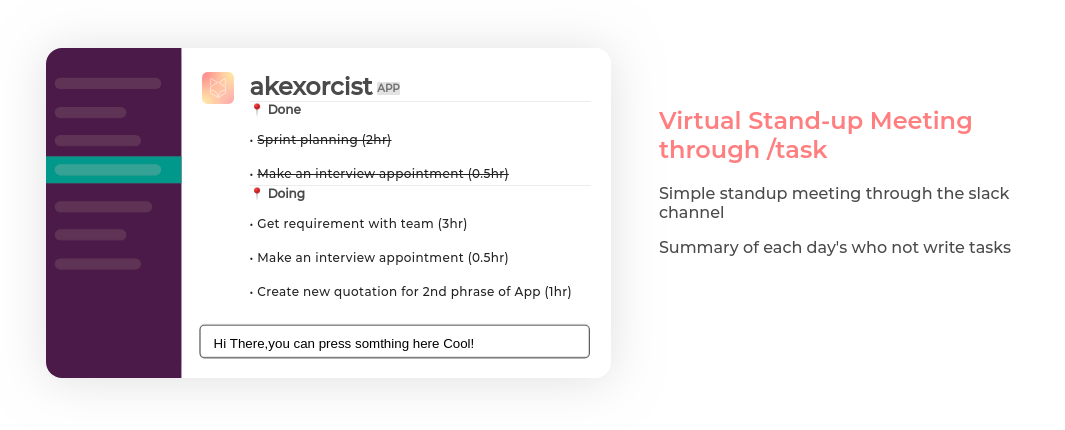
\includegraphics[width=0.7\linewidth]{landing-page-5}
		\label{Fig:landing-page-5}
	}
	\subfigure[Section-6]{
		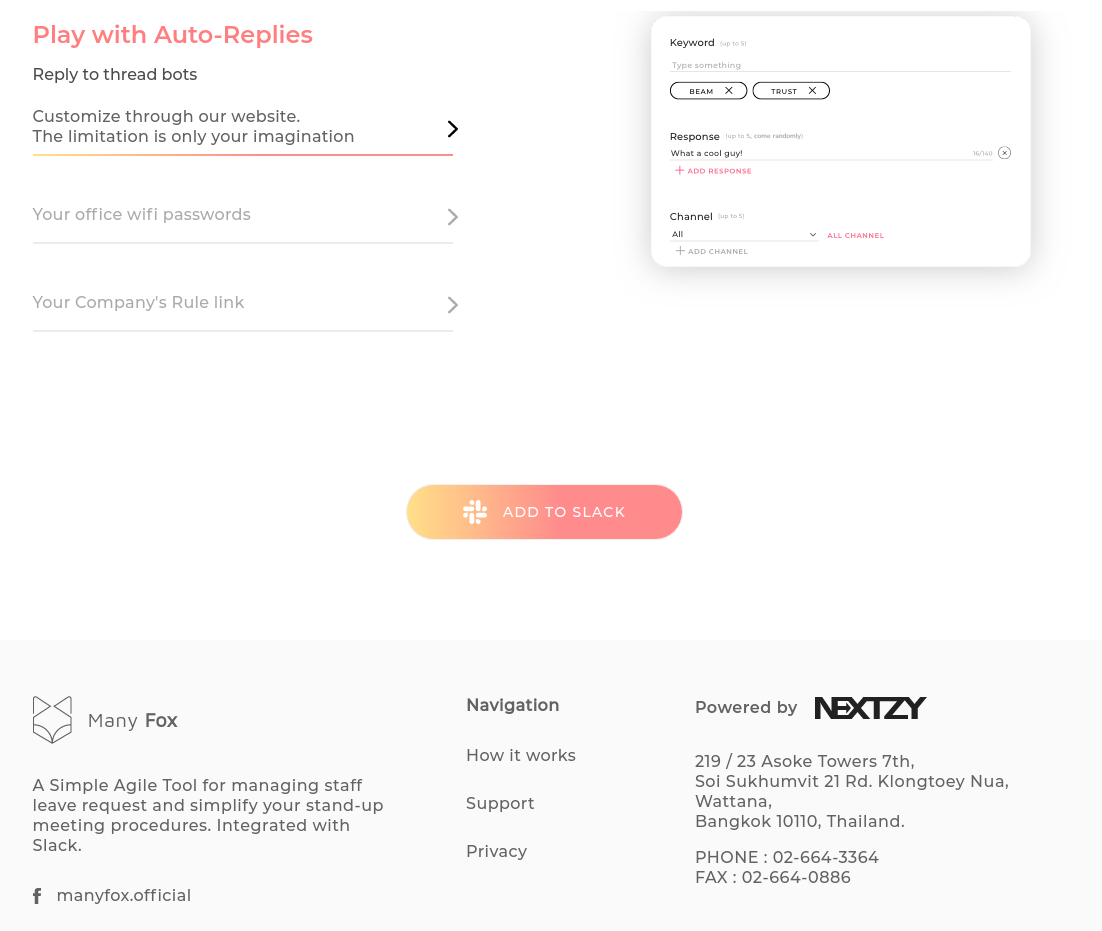
\includegraphics[width=0.7\linewidth]{landing-page-6}
		\label{Fig:landing-page-6}
	}
	\caption{Landing page}
\end{figure}